\documentclass[t,aspectratio=169]{beamer}
\usetheme{default}

\usepackage{cmap}
\usepackage[T2A]{fontenc}
\usepackage[utf8]{inputenc}
\usepackage[english,russian]{babel}
\usepackage{amsmath,amsfonts,amssymb,mathtools}
\usepackage{graphicx}
\usepackage{booktabs}
\usepackage{tabularx}
\usepackage{tikz}
\usepackage{capt-of}
\usepackage{hyperref}

\usetikzlibrary{arrows.meta,positioning,calc}
\graphicspath{{images/}}

\hypersetup{
  unicode=true,
  colorlinks=true,
  linkcolor=black,
  urlcolor=blue
}

\setbeamertemplate{navigation symbols}{}
\setbeamertemplate{footline}[frame number]
\setbeamertemplate{itemize item}{\(\blacktriangleright\)}
\setbeamertemplate{itemize subitem}{\(\triangleright\)}
\setbeamerfont{frametitle}{size=\large}
\setbeamerfont{framesubtitle}{size=\small}
\setbeamerfont{footline}{size=\scriptsize}
\setbeamerfont{block title}{size=\small}
\setbeamerfont{block body}{size=\scriptsize}
\setbeamercolor{block title}{fg=black,bg=gray!15}
\setbeamercolor{block body}{fg=black,bg=gray!6}

\newcommand{\E}{\mathcal E}
\newcommand{\Usaw}{\mathcal U}
\newcommand{\R}{\mathcal R}
\newcommand{\source}[1]{\vfill{\tiny\raggedright #1\par}}
\newcommand{\twopics}[4]{
  \begin{columns}[T,onlytextwidth]
    \column{0.5\textwidth}
    \centering
    \includegraphics[width=#1\linewidth]{#2}
    \column{0.5\textwidth}
    \centering
    \includegraphics[width=#3\linewidth]{#4}
  \end{columns}
}

\title{Численное исследование спиновых моделей на динамических структурах}
\subtitle{Модель Изинга и XY-модель на блужданиях без самопересечений}
\author{Файзуллина Камилла}
\institute{Научный руководитель: Л.Н. Щур}
\date{}

\begin{document}

\begin{frame}[plain]
  \titlepage
\end{frame}

\section{Классические модели и переходы}

\begin{frame}{Модель Изинга: дискретная симметрия}
  \begin{columns}[T,onlytextwidth]
    \column{0.44\textwidth}
    \small
    \[
      H_{\mathrm{Ising}}
      = -J\sum_{\langle i,j\rangle} s_i s_j,\qquad
      s_i=\pm1 .
    \]
    \begin{itemize}
      \item Параметр порядка: \(m=N^{-1}\sum_i s_i\).
      \item В 2D на квадратной решетке есть точное решение.
      \item При \(T<T_c\): ферромагнитный порядок.
      \item При \(T>T_c\): парамагнитный режим.
    \end{itemize}
    \column{0.48\textwidth}
    \centering
    \begin{tikzpicture}[scale=0.75]
      \foreach \x in {0,...,5}{
        \foreach \y in {0,...,4}{
          \draw[gray!35] (\x,\y) -- ++(1,0);
          \draw[gray!35] (\x,\y) -- ++(0,1);
        }
      }
      \foreach \x in {0,...,6}{
        \foreach \y in {0,...,5}{
          \pgfmathtruncatemacro{\up}{mod(\x+\y,3)}
          \ifnum\up=0
            \draw[very thick,blue!70!black,-{Latex[length=2mm]}] (\x,\y-0.22) -- (\x,\y+0.22);
          \else
            \draw[very thick,red!70!black,-{Latex[length=2mm]}] (\x,\y+0.22) -- (\x,\y-0.22);
          \fi
        }
      }
      \node[font=\scriptsize] at (3,-0.7) {локальные взаимодействия ближайших соседей};
    \end{tikzpicture}
  \end{columns}
  \source{E. Ising, Z. Phys. 31, 253--258 (1925); L. Onsager, Phys. Rev. 65, 117--149 (1944).}
\end{frame}

\begin{frame}{XY-модель: непрерывная симметрия}
  \begin{columns}[T,onlytextwidth]
    \column{0.52\textwidth}
    \small
    \[
      \begin{aligned}
        H_{XY}&=-J\sum_{\langle i,j\rangle}\cos(\theta_i-\theta_j),\\
        \vec s_i&=(\cos\theta_i,\sin\theta_i).
      \end{aligned}
    \]
    \begin{itemize}
      \item Симметрия \(O(2)\), параметр порядка в конечной системе:
      \[
        m=\frac{1}{N}\sqrt{\left(\sum_i\cos\theta_i\right)^2+
        \left(\sum_i\sin\theta_i\right)^2}.
      \]
      \item В 2D обычного дальнего порядка нет.
      \item Вместо обычного перехода возникает БКТ-сценарий.
    \end{itemize}
    \column{0.48\textwidth}
    \centering
    \begin{tikzpicture}[scale=0.75]
      \foreach \x in {0,...,6}{
        \foreach \y in {0,...,5}{
          \fill[gray!25] (\x,\y) circle (0.025);
          \pgfmathsetmacro{\ang}{25*\x+35*\y+10*sin(30*\x)}
          \draw[very thick,teal!70!black,-{Latex[length=2mm]}]
            (\x,\y) -- ++(\ang:0.35);
        }
      }
      \node[font=\scriptsize] at (3,-0.7) {угловые степени свободы};
    \end{tikzpicture}
  \end{columns}
  \source{J. M. Kosterlitz and D. J. Thouless, J. Phys. C 6, 1181 (1973); В. Л. Березинский, ЖЭТФ (1970, 1971).}
\end{frame}

\begin{frame}{БКТ-переход: не обычная критическая точка}
  \small
  \begin{columns}[T,onlytextwidth]
    \column{0.46\textwidth}
    \begin{block}{Физическая картина}
      \begin{itemize}
        \item При низких \(T\): связанные пары вихрь-антивихрь.
        \item При высоких \(T\): свободные вихри разрушают квазидальний порядок.
        \item Корреляционная длина расходится экспоненциально, а не степенно.
      \end{itemize}
    \end{block}
    \[
      G(r)\sim r^{-\eta},\qquad
      \eta(T_{\mathrm{BKT}})=\frac14.
    \]
    \[
      \xi \sim \exp\!\left(\frac{b}{\sqrt{|T-T_{\mathrm{BKT}}|}}\right).
    \]
    \column{0.50\textwidth}
    \centering
    \begin{tikzpicture}[scale=0.86]
      \draw[->] (0,0) -- (5.6,0) node[right] {\scriptsize \(T\)};
      \draw[->] (0,0) -- (0,3.3) node[above] {\scriptsize корреляции};
      \draw[thick,teal!70!black] (0.3,2.7) .. controls (1.5,2.4) and (2.5,1.8) .. (3.1,0.9);
      \draw[thick,red!70!black] (3.1,0.9) .. controls (3.7,0.35) and (4.7,0.18) .. (5.2,0.13);
      \draw[dashed] (3.1,0) -- (3.1,3.0);
      \node[font=\scriptsize] at (3.1,-0.35) {\(T_{\mathrm{BKT}}\)};
      \node[font=\scriptsize,align=center] at (1.4,0.75) {квазидальний\\порядок};
      \node[font=\scriptsize,align=center] at (4.45,0.75) {экспоненциальный\\спад};
      \draw[blue!70!black,thick] (1.1,2.2) circle (0.35);
      \draw[blue!70!black,thick] (1.8,2.2) circle (0.35);
      \node[font=\scriptsize] at (1.45,2.8) {пара};
      \draw[red!70!black,thick] (4.1,2.15) circle (0.35);
      \draw[red!70!black,thick] (5.0,1.65) circle (0.35);
      \node[font=\scriptsize] at (4.55,2.75) {свободные вихри};
    \end{tikzpicture}
  \end{columns}
\end{frame}

\begin{frame}{Полимер: блуждание без самопересечений}
  \begin{columns}[T,onlytextwidth]
    \column{0.5\textwidth}
    \small
    Геометрия линейного полимера длины \(N\) задается БСП:
    \[
      u=(r_1,\dots,r_N),\qquad r_i\ne r_j \ (i\ne j).
    \]
    Размер цепи:
    \[
      \langle R_N^2\rangle \sim N^{2\nu}.
    \]
    \begin{tabular}{@{}lcc@{}}
      \toprule
      режим & 2D & 3D \\
      \midrule
      хорош. растворитель & \(3/4\) & \(\simeq0.588\) \\
      \(\Theta\)-точка & \(4/7\) & \(1/2\) \\
      глобула & \(1/2\) & \(1/3\) \\
      \bottomrule
    \end{tabular}
    \column{0.5\textwidth}
    \centering
    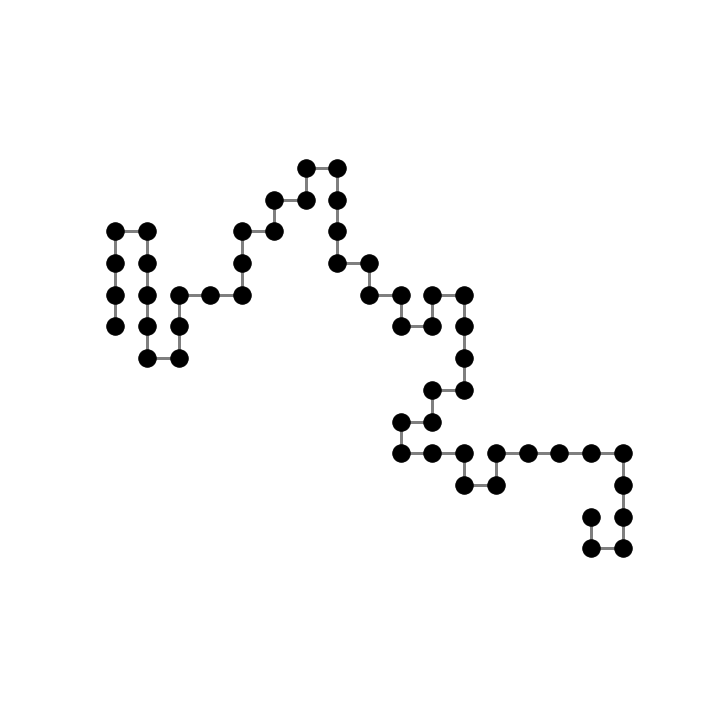
\includegraphics[width=0.6\linewidth]{homopolymer.png}
    \vspace{0.5em}

    \scriptsize
    Переход клубок-глобула:
    \[
      \frac{\langle R_N^2\rangle}{N^{2\nu_\Theta}}
      =
      \R\!\left((J-J_\Theta)N^{\phi_\Theta}\right).
    \]
  \end{columns}
  \source{P.-G. de Gennes, Scaling Concepts in Polymer Physics (1979); Duplantier and Saleur, Phys. Rev. Lett. 59, 539 (1987).}
\end{frame}

\section{Обзор разработанности темы}

\begin{frame}{От регулярной решетки к динамическому графу}
  \small
  \begin{columns}[T,onlytextwidth]
    \column{0.50\textwidth}
    \begin{block}{Фиксированная решетка}
      \[
        H=-J\sum_{\langle i,j\rangle\in\E_0}e_{ij}.
      \]
      Граф \(\E_0\) задан заранее. Вопрос: как симметрия спина и размерность решетки определяют переход?
    \end{block}
    \begin{block}{БСП как носитель}
      \[
        H(u,s)=-J\sum_{\langle i,j\rangle\in\E(u)}e_{ij}.
      \]
      Граф \(\E(u)\) меняется вместе с конформацией цепи.
    \end{block}
    \column{0.46\textwidth}
    \begin{itemize}
      \item На регулярных решетках Изинг и XY являются эталонными моделями фазовых переходов.
      \item На БСП сама геометрия становится термодинамической переменной.
      \item Главный вопрос семинара: когда магнитное упорядочение ведет за собой коллапс цепи, а когда эти процессы расходятся?
    \end{itemize}
  \end{columns}
  \source{Chakrabarti and Bhattacharya, J. Phys. C 16, L1025 (1983); Chakrabarti, Maggs and Stinchcombe, J. Phys. A 18, L373 (1985).}
\end{frame}

\begin{frame}{Изинг на БСП: что было известно}
  \small
  \[
    H(u,\sigma)=-J\sum_{\langle i,j\rangle\in\E(u)}\sigma_i\sigma_j,
    \qquad \sigma_i=\pm1.
  \]
  \begin{itemize}
    \item Первые работы рассматривали Изинг на БСП как способ уйти от фиксированной решетки к полимерному носителю.
    \item В 3D по Garel--Orland--Orlandini магнитно-индуцированный коллапс и намагничивание идут вместе; сценарий первого рода.
    \item Foster--Majumdar и наши данные показывают, что в 2D переход непрерывный, а структурная и магнитная области совпадают в пределах численной точности.
    \item Поэтому Изинг здесь не конечная остановка, а контрольный дискретный случай перед непрерывной XY-симметрией.
  \end{itemize}
  \vspace{0.4em}
  \source{Garel, Orland and Orlandini, EPJ B 12, 261--268 (1999); Foster and Majumdar, Phys. Rev. E 104, 024122 (2021); Faizullina, Pchelintsev and Burovski, Phys. Rev. E 104, 054501 (2021).}
\end{frame}

\begin{frame}{Potts-полимеры: попытка привязки к хроматину}
  \small
  В моделях хроматина внутреннее состояние мономера трактуется как эпигенетическая метка. Минимальная статистико-механическая версия: \(q\)-состояния Potts-типа на полимерной цепи.
  \[
    H(u,\sigma)=
    -J\sum_{\langle i,j\rangle\in\E(u)}\delta_{\sigma_i,\sigma_j}
    +\Delta\sum_{i=1}^{N}\sigma_i^2,
    \qquad \sigma_i\in\{1,\ldots,q\}.
  \]
  \begin{itemize}
    \item Цепь сворачивается за счет контактов мономеров с одинаковыми метками.
    \item Параметр \(\Delta\) позволяет стабилизировать компактную, но неупорядоченную фазу.
    \item Это важный контекст: даже дискретные внутренние переменные уже дают не одну линию перехода, а фазовую диаграмму.
  \end{itemize}
  \source{Colì, Orlandini, Michieletto and Marenduzzo, Phys. Rev. E 100, 052410 (2019); Nakanishi and Hukushima, Phys. Rev. E 109, 014405 (2024).}
\end{frame}

\begin{frame}{BEG и двухблочные расширения}
  \small
  \[
    H =
    -\frac{J}{2}\sum_{i,j}S_i\Lambda_{ij}S_j
    -\frac{K}{2}\sum_{i,j}S_i^2\Lambda_{ij}S_j^2
    +\Delta\sum_i S_i^2,\qquad S_i\in\{-1,0,1\}.
  \]
  \begin{itemize}
    \item Итальянская линия работ по BEG-полимерам показывает три фазы: swollen disordered, compact ordered, compact disordered.
    \item Мультикритические точки двигаются при изменении \(K/J\) и \(\Delta\); это уже не просто «коллапс плюс магнитный порядок».
    \item В двухблочных расширениях конкурируют взаимодействия внутри блоков и между блоками, что ближе к гетерогенным полимерам и хроматину.
    \item Но все эти модели остаются дискретными; непрерывная \(O(2)\)-симметрия остается отдельным вопросом.
  \end{itemize}
  \source{Raiola, Locatelli, Marenduzzo and Orlandini, Soft Matter 21, 5296--5311 (2025).}
\end{frame}

\section{Модели и методы}

\begin{frame}{Общая постановка}
  \small
  Полимерная конфигурация \(u\) задает контактный граф \(\E(u)\). Спины живут на мономерах, а энергия вычисляется не на фиксированной решетке, а на графе текущей конформации.
  \[
    Z_N(J)=\sum_{u\in\Usaw_N}\sum_{s\in\mathcal S}
    \exp\!\left[J\sum_{(i,j)\in\E(u)} e_{ij}\right].
  \]
  \begin{columns}[T,onlytextwidth]
    \column{0.48\textwidth}
    \begin{block}{Модель Изинга}
      \[
        e_{ij}=s_i s_j,\qquad s_i=\pm1.
      \]
      Дискретная симметрия, обычный параметр порядка \(m\).
    \end{block}
    \column{0.48\textwidth}
    \begin{block}{XY-модель}
      \[
        e_{ij}=\cos(\theta_i-\theta_j),\qquad \theta_i\in(-\pi,\pi].
      \]
      Непрерывная симметрия, в 2D ожидается БКТ-подобная логика.
    \end{block}
  \end{columns}
  \source{Faizullina, Pchelintsev and Burovski, Phys. Rev. E 104, 054501 (2021); Faizullina and Burovski, Phys. Rev. E 112, 024107 (2025).}
\end{frame}

\begin{frame}{Что именно входит в сумму по контактам}
  \begin{columns}[T,onlytextwidth]
    \column{0.50\textwidth}
    \small
    \[
      \E(u)=
      \{(i,j): |r_i-r_j|=1,\ |i-j|>1\}.
    \]
    \[
      C(u)=|\E(u)|.
    \]
    \begin{itemize}
      \item \(u=(r_1,\ldots,r_N)\) --- самонепересекающаяся цепочка на квадратной или кубической решетке.
      \item \(\E(u)\) содержит пространственные контакты мономеров, которые оказались соседями на решетке.
      \item \(C(u)\) затем используется как геометрическая наблюдаемая: он растет при сворачивании цепи.
    \end{itemize}
    \column{0.50\textwidth}
    \centering
    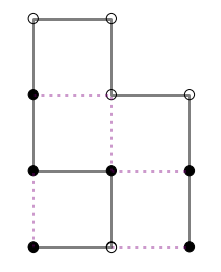
\includegraphics[width=0.60\linewidth]{onlysaw.png}
  \end{columns}
\end{frame}

\begin{frame}{Канонический алгоритм: 1. змееподобный шаг}
  \small
  \begin{columns}[T,onlytextwidth]
    \column{0.48\textwidth}
    Предложение нового состояния:
    \[
      (u,s)\to(v,s'),\qquad
      \Delta H=H(v,s')-H(u,s).
    \]
    \[
      A(u\to v)=
      \min\{1,\exp[-\Delta H]\}.
    \]
    \begin{itemize}
      \item Удаляется один конец цепи.
      \item На другом конце пробуется новый шаг в допустимом направлении.
      \item Для нового мономера выбирается новый спин: \(s_i=\pm1\) или \(\theta_i\in(-\pi,\pi]\).
    \end{itemize}
    \column{0.48\textwidth}
    \centering
    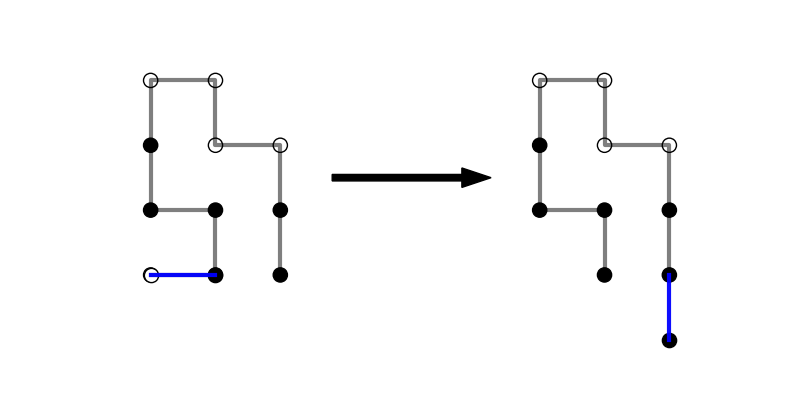
\includegraphics[width=0.88\linewidth]{snakeupdate.png}
  \end{columns}
\end{frame}

\begin{frame}{Канонический алгоритм: 2. смена соединений}
  \small
  \begin{columns}[T,onlytextwidth]
    \column{0.48\textwidth}
    \begin{itemize}
      \item Шаг меняет порядок соединения мономеров при фиксированных координатах.
      \item Условие самонепересечения сохраняется.
      \item Такой ход ускоряет перестройку геометрии цепи.
    \end{itemize}
    \[
      A(u\to v)=
      \begin{cases}
        1, & \text{если } v\in\Usaw_N,\\
        0, & \text{иначе.}
      \end{cases}
    \]
    В этой операции координаты и спины не меняются; меняется только то, какие узлы считаются последовательными вдоль цепи.
    \column{0.52\textwidth}
    \centering
    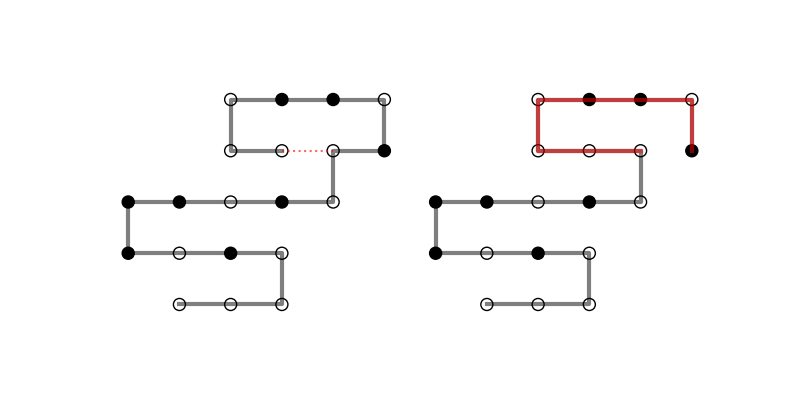
\includegraphics[width=0.92\linewidth]{reconnect.png}
  \end{columns}
  \source{Prokof'ev and Svistunov, Phys. Rev. Lett. 87, 160601 (2001).}
\end{frame}

\begin{frame}{Канонический алгоритм: 3. кластерный шаг}
  \small
  \begin{columns}[T,onlytextwidth]
    \column{0.48\textwidth}
    \[
      P_{\mathrm{add}}(\vec S_i,\vec S_j)
      =
      1-\exp\!\left[-2J(\vec S_i\vec n)(\vec S_j\vec n)\right].
    \]
    \begin{itemize}
      \item Для XY выбирается случайное направление \(\vec n\).
      \item Кластер отражается относительно плоскости, перпендикулярной \(\vec n\).
      \item Для Изинга сосед добавляется при \(s_i=s_j\) с вероятностью \(1-e^{-2J}\), затем весь кластер переворачивается.
    \end{itemize}
    \column{0.52\textwidth}
    \centering
    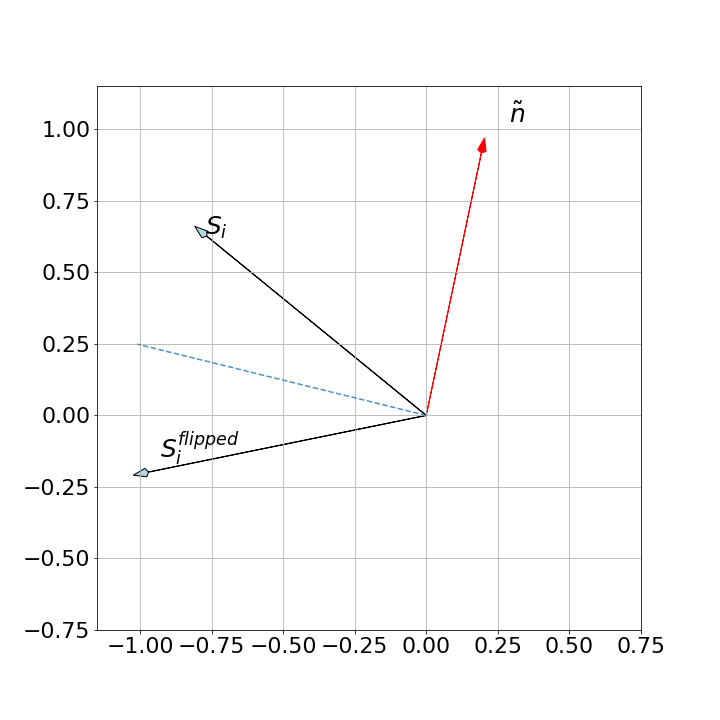
\includegraphics[width=0.48\linewidth]{cluster_flip.png}
    \includegraphics[width=0.48\linewidth]{state_example_cluster.png}
  \end{columns}
  \source{Wolff, Phys. Rev. Lett. 62, 361--364 (1989).}
\end{frame}

\begin{frame}{Второй набор данных: обмен репликами}
  \small
  Прямые прогоны выполнялись независимо при фиксированных \((N,J)\). Второй набор данных строился отдельно: несколько реплик одной системы моделируются при сетке
  \[
    J_1<J_2<\ldots<J_M .
  \]
  Периодически пробуется обмен состояниями соседних реплик:
  \[
    (u_m,s_m,J_m)\leftrightarrow(u_{m+1},s_{m+1},J_{m+1}).
  \]
  \[
    A_{\mathrm{swap}}=
    \min\!\left\{1,
    \exp\!\left[(J_m-J_{m+1})(E_m-E_{m+1})\right]\right\}.
  \]
  \begin{itemize}
    \item Это не замена прямых данных, а независимая проверка в узкой переходной области.
    \item Сетка \(J_m\) выбирается так, чтобы соседние энергетические гистограммы перекрывались.
    \item Обмен помогает траекториям проходить между развернутыми и компактными состояниями.
  \end{itemize}
\end{frame}

\begin{frame}{Мультигистограммное перевзвешивание}
  \small
  Для каждой конфигурации удобно выделить
  \[
    Q(u,s)=\sum_{(i,j)\in\E(u)}e_{ij},\qquad H=-JQ.
  \]
  Тогда для близких значений \(J\) гистограммы по \(Q\) дают оценку плотности состояний \(\Omega(Q)\):
  \[
    P_J(Q)\propto \Omega(Q)e^{JQ},
    \qquad
    \langle O\rangle_J=
    \frac{\sum_Q \overline O(Q)\Omega(Q)e^{JQ}}
    {\sum_Q \Omega(Q)e^{JQ}}.
  \]
  \begin{columns}[T,onlytextwidth]
    \column{0.48\textwidth}
    \begin{itemize}
      \item строятся гладкие зависимости \(R^2(J)\), \(U_4(J)\), \(c_V(J)\);
      \item уточняются пересечения и псевдокритические точки;
      \item оцениваются конечномерные поправки.
    \end{itemize}
    \column{0.48\textwidth}
    \[
      c_V(J)=\frac{1}{N}\left(\langle H^2\rangle-\langle H\rangle^2\right).
    \]
    \[
      U_4=1-\frac{\langle m^4\rangle}{3\langle m^2\rangle^2}.
    \]
    \[
      \frac{\langle R_N^2\rangle}{N^{2\nu_\Theta}}
      =
      \R\!\left((J-J_\Theta)N^{\phi_\Theta}\right).
    \]
  \end{columns}
  \source{Swendsen and Wang, Phys. Rev. Lett. 57, 2607 (1986); Ferrenberg and Swendsen, Phys. Rev. Lett. 63, 1195 (1989).}
\end{frame}

\begin{frame}{Корреляции геометрии и магнетизма}
  \small
  На каждом состоянии измеряются две величины: число пространственных контактов \(C\) и модуль намагниченности \(|m|\). Их совместная статистика показывает, происходят ли компактизация и магнитное упорядочение в одних и тех же конфигурациях.
  \[
    \mathrm{Cov}_J(C,|m|)
    =
    \langle C|m|\rangle_J-\langle C\rangle_J\langle |m|\rangle_J .
  \]
  \[
    \rho_P(J)=
    \frac{\mathrm{Cov}_J(C,|m|)}
    {\sqrt{\mathrm{Var}_J(C)\mathrm{Var}_J(|m|)}}.
  \]
  \[
    \rho_S(J)=\rho_P(R_C,R_m),
  \]
  где \(R_C\) и \(R_m\) --- ранги \(C\) и \(|m|\) в выборке при фиксированном \(J\).
  \begin{block}{Как это читать}
    \(\rho\simeq1\): более компактные состояния почти всегда более намагничены. \(\rho\simeq0\): геометрия и магнитный порядок в этой области слабо связаны.
  \end{block}
\end{frame}

\section{Модель Изинга на БСП}

\begin{frame}{Модель Изинга на БСП}
  \small
  \begin{columns}[T,onlytextwidth]
    \column{0.50\textwidth}
    \[
      H(u,s)=-J\sum_{\langle i,j\rangle\in\E(u)}s_i s_j,
      \qquad s_i=\pm1.
    \]
    \[
      Z_N(J)=
      \sum_{u\in\Usaw_N}\sum_{s\in\{\pm1\}^N}
      \exp\!\left[J\sum_{(i,j)\in\E(u)}s_i s_j\right].
    \]
    \begin{itemize}
      \item Геометрия \(u\) является частью статистической суммы.
      \item Спины взаимодействуют только через пространственные контакты \(\E(u)\).
    \end{itemize}
    \column{0.48\textwidth}
    \centering
    \includegraphics[width=0.96\linewidth]{ising_polymer_examples.png}
    \vspace{0.3em}

    \scriptsize
    Чёрные/белые узлы: \(s_i=\pm1\). Геометрия и спины обновляются совместно.
  \end{columns}
  \source{Faizullina, Pchelintsev and Burovski, Phys. Rev. E 104, 054501 (2021).}
\end{frame}

\begin{frame}{Изинг 2D: геометрический переход}
  \small
  \[
    \frac{\langle R_N^2\rangle}{N^{2\nu_\Theta}}
    =
    \R((J-J_\Theta)N^{\phi_\Theta}),
    \qquad
    \nu_\Theta=\frac47.
  \]
  \begin{columns}[T,onlytextwidth]
    \column{0.55\textwidth}
    \centering
    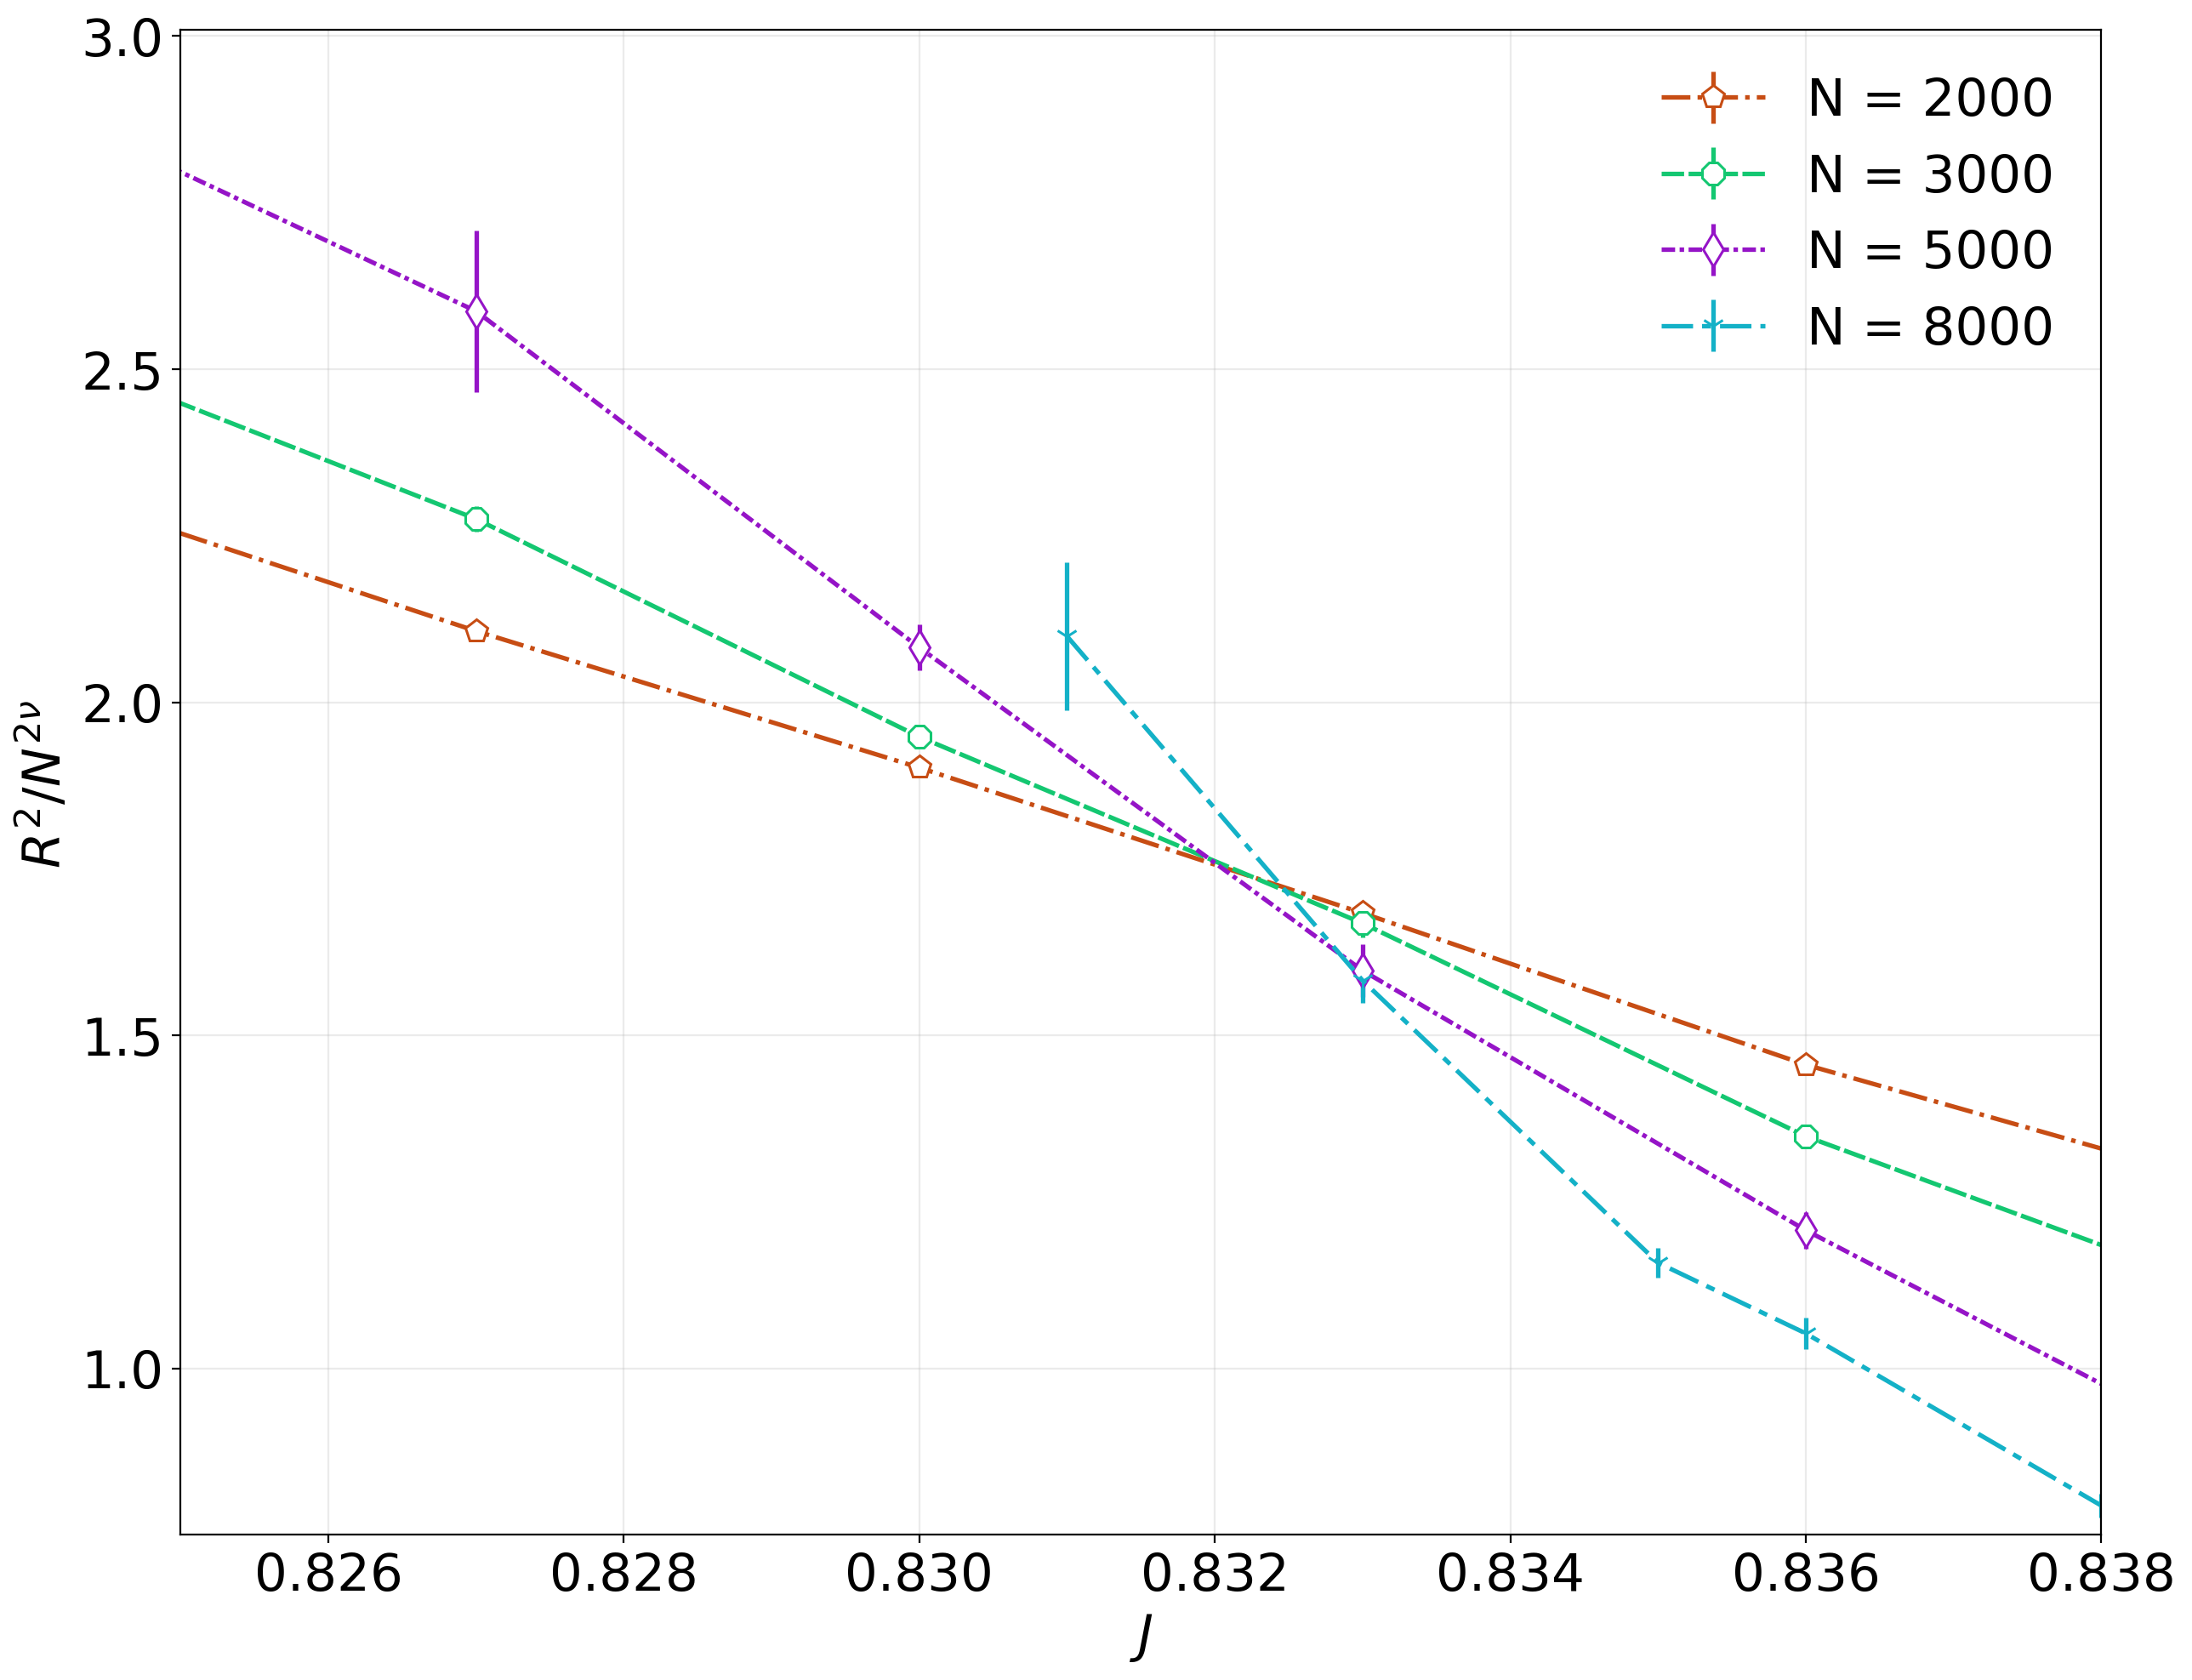
\includegraphics[width=0.95\linewidth]{Ising_2D_rscaling_long_fixed.png}
    \column{0.45\textwidth}
    \begin{block}{Оценка}
      \[
        J_\Theta \approx 0.833(1).
      \]
    \end{block}
    \begin{itemize}
      \item Отмасштабированные радиусы пересекаются в узкой области.
      \item Критический показатель \(\nu_\Theta=4/7\) наследуется от родительского \(\Theta\)-полимера.
      \item Переход геометрически непрерывный.
    \end{itemize}
  \end{columns}
\end{frame}

\begin{frame}{Изинг 2D: магнитный переход}
  \small
  \begin{columns}[T,onlytextwidth]
    \column{0.52\textwidth}
    \centering
    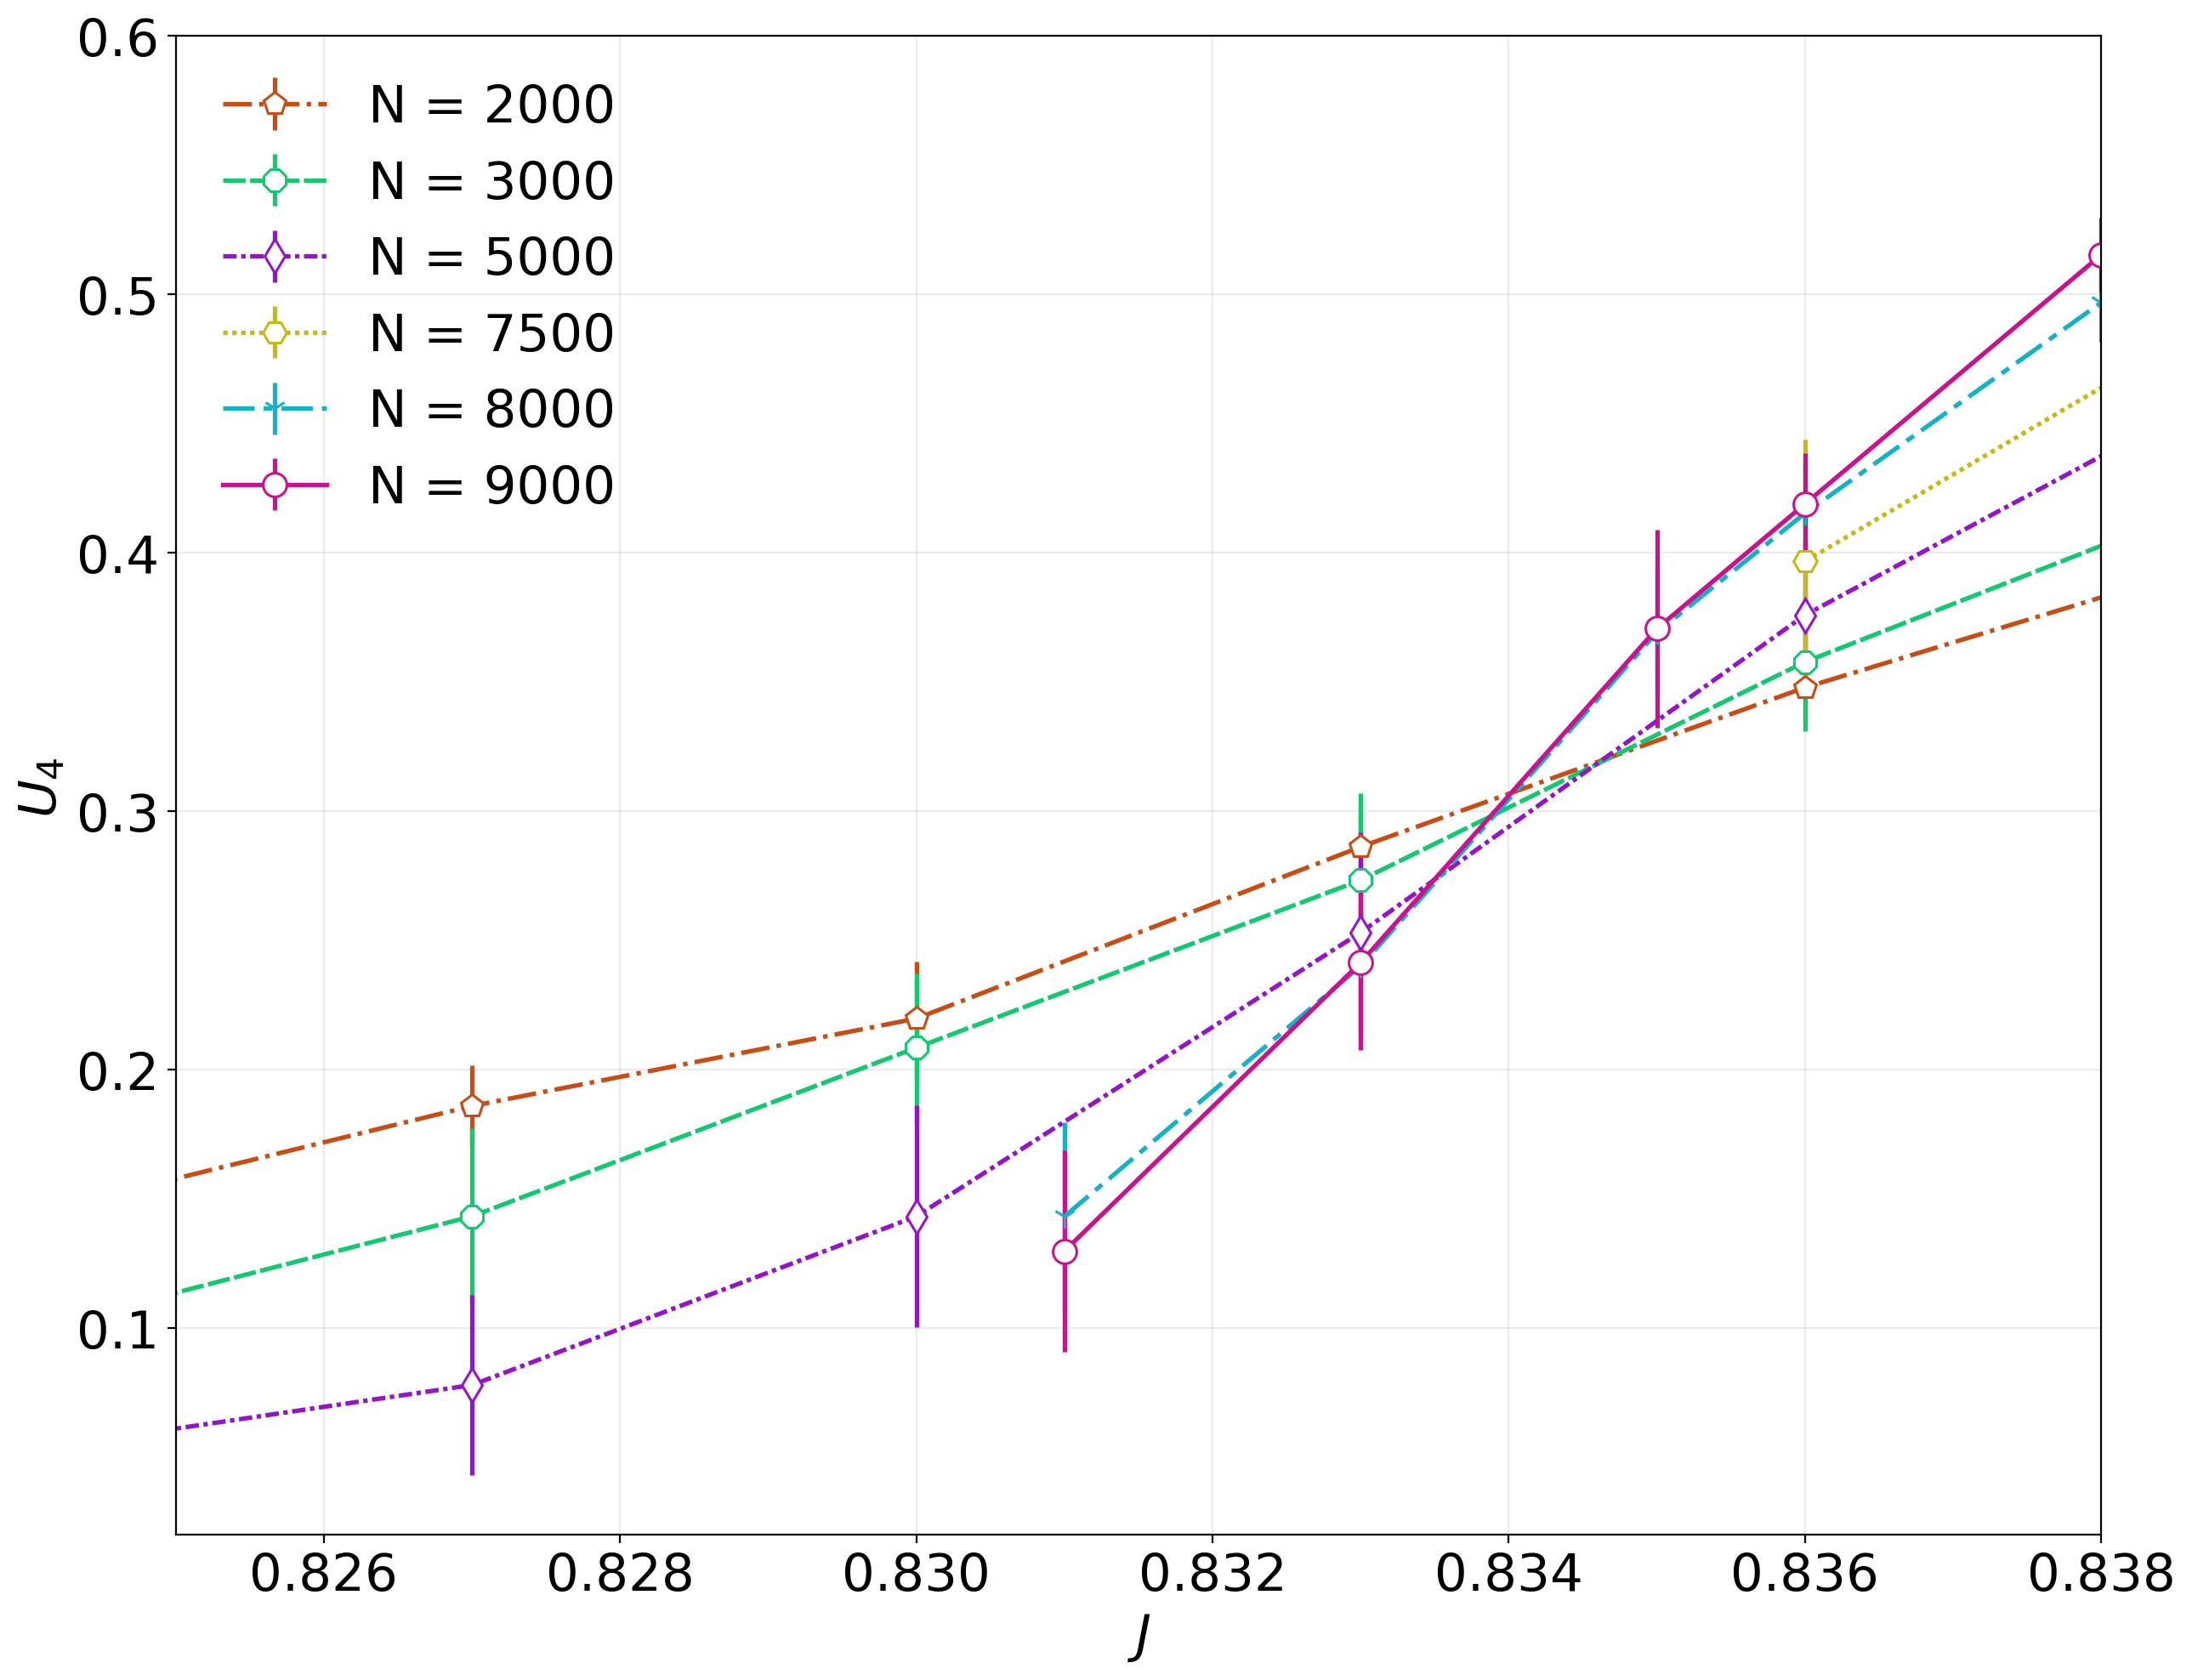
\includegraphics[width=\linewidth]{Ising_2D_U4_long_fixed.png}
    \column{0.48\textwidth}
    \[
      U_4=1-\frac{\langle m^4\rangle}
      {3\langle m^2\rangle^2}.
    \]
    \begin{block}{Оценки}
      \[
        J_{\mathrm{cr}}=0.8340(5)
      \]
      по прямым данным.
    \end{block}
    \begin{itemize}
      \item Кривые \(U_4\) пересекаются.
      \item Отрицательного провала нет.
      \item Магнитный переход непрерывный.
    \end{itemize}
  \end{columns}
\end{frame}

\begin{frame}{Изинг 2D: распределение энергии}
  \small
  \[
    H(u,s)=-J\sum_{\langle i,j\rangle\in\E(u)}s_i s_j,
    \qquad e=H/N .
  \]
  \centering
  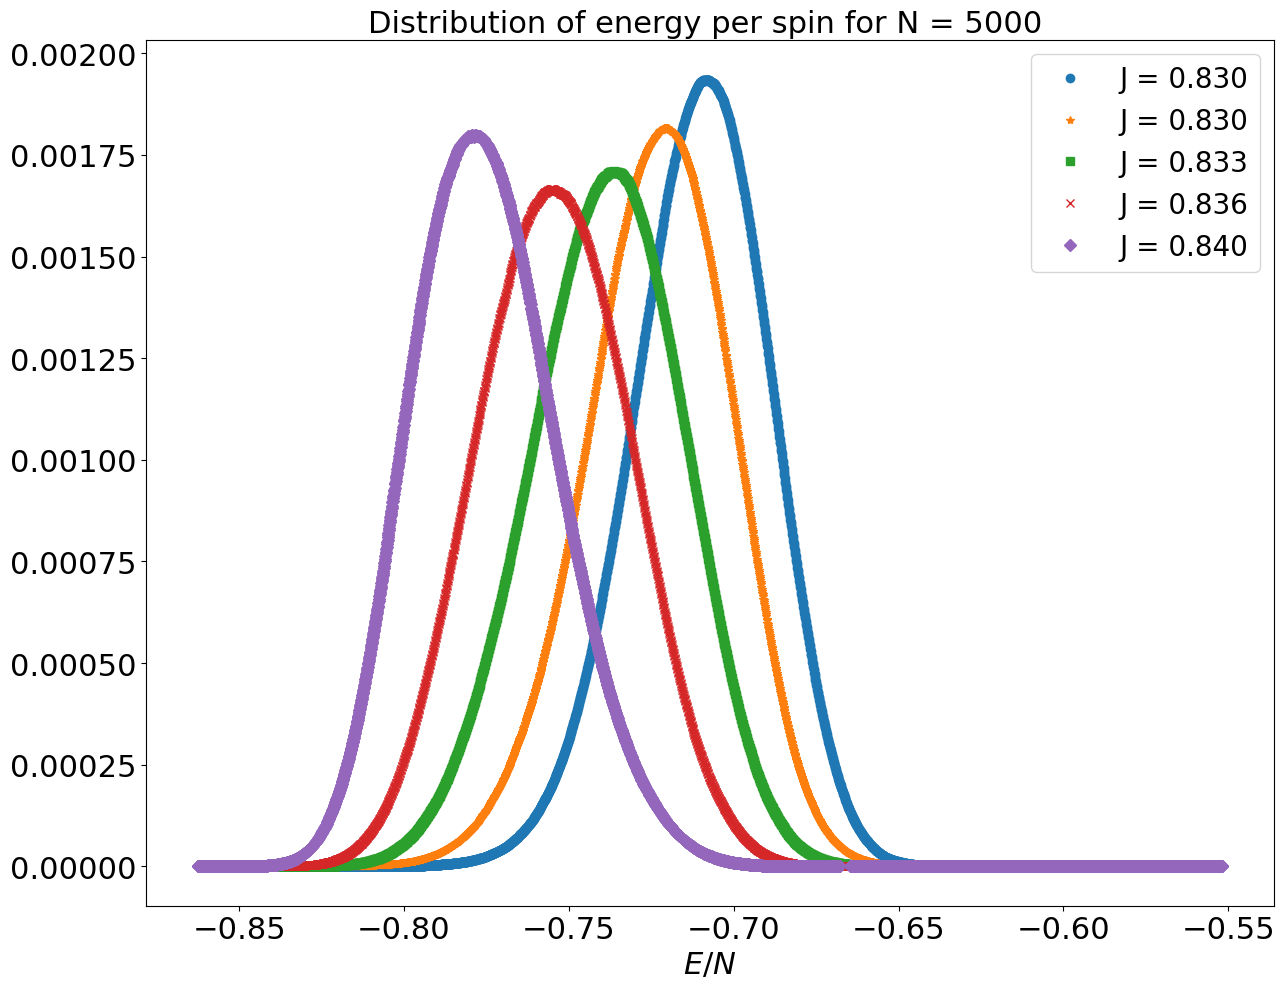
\includegraphics[width=0.70\linewidth,height=0.60\textheight,keepaspectratio]{Ising_distrenergy_5000.png}

  \vspace{0.2em}
  \scriptsize
  \(N=5000\). Одномодальная форма в переходной области: нет видимого сосуществования энергетических фаз.
\end{frame}

\begin{frame}{Изинг 2D: триптих распределений}
  \centering
  \includegraphics[width=0.98\textwidth,height=0.78\textheight,keepaspectratio]{triptych_L_Ising_SI_2D_7000.png}

  {\scriptsize \(N=7000\). Слева направо: \(P(e)\), \(P(|m|)\), \(P(C/N)\); все три распределения остаются одномодальными.}
\end{frame}

\begin{frame}{Изинг 2D: анализ перевзвешенных данных}
  \scriptsize
  \begin{columns}[T,onlytextwidth]
    \column{0.50\textwidth}
    \centering
    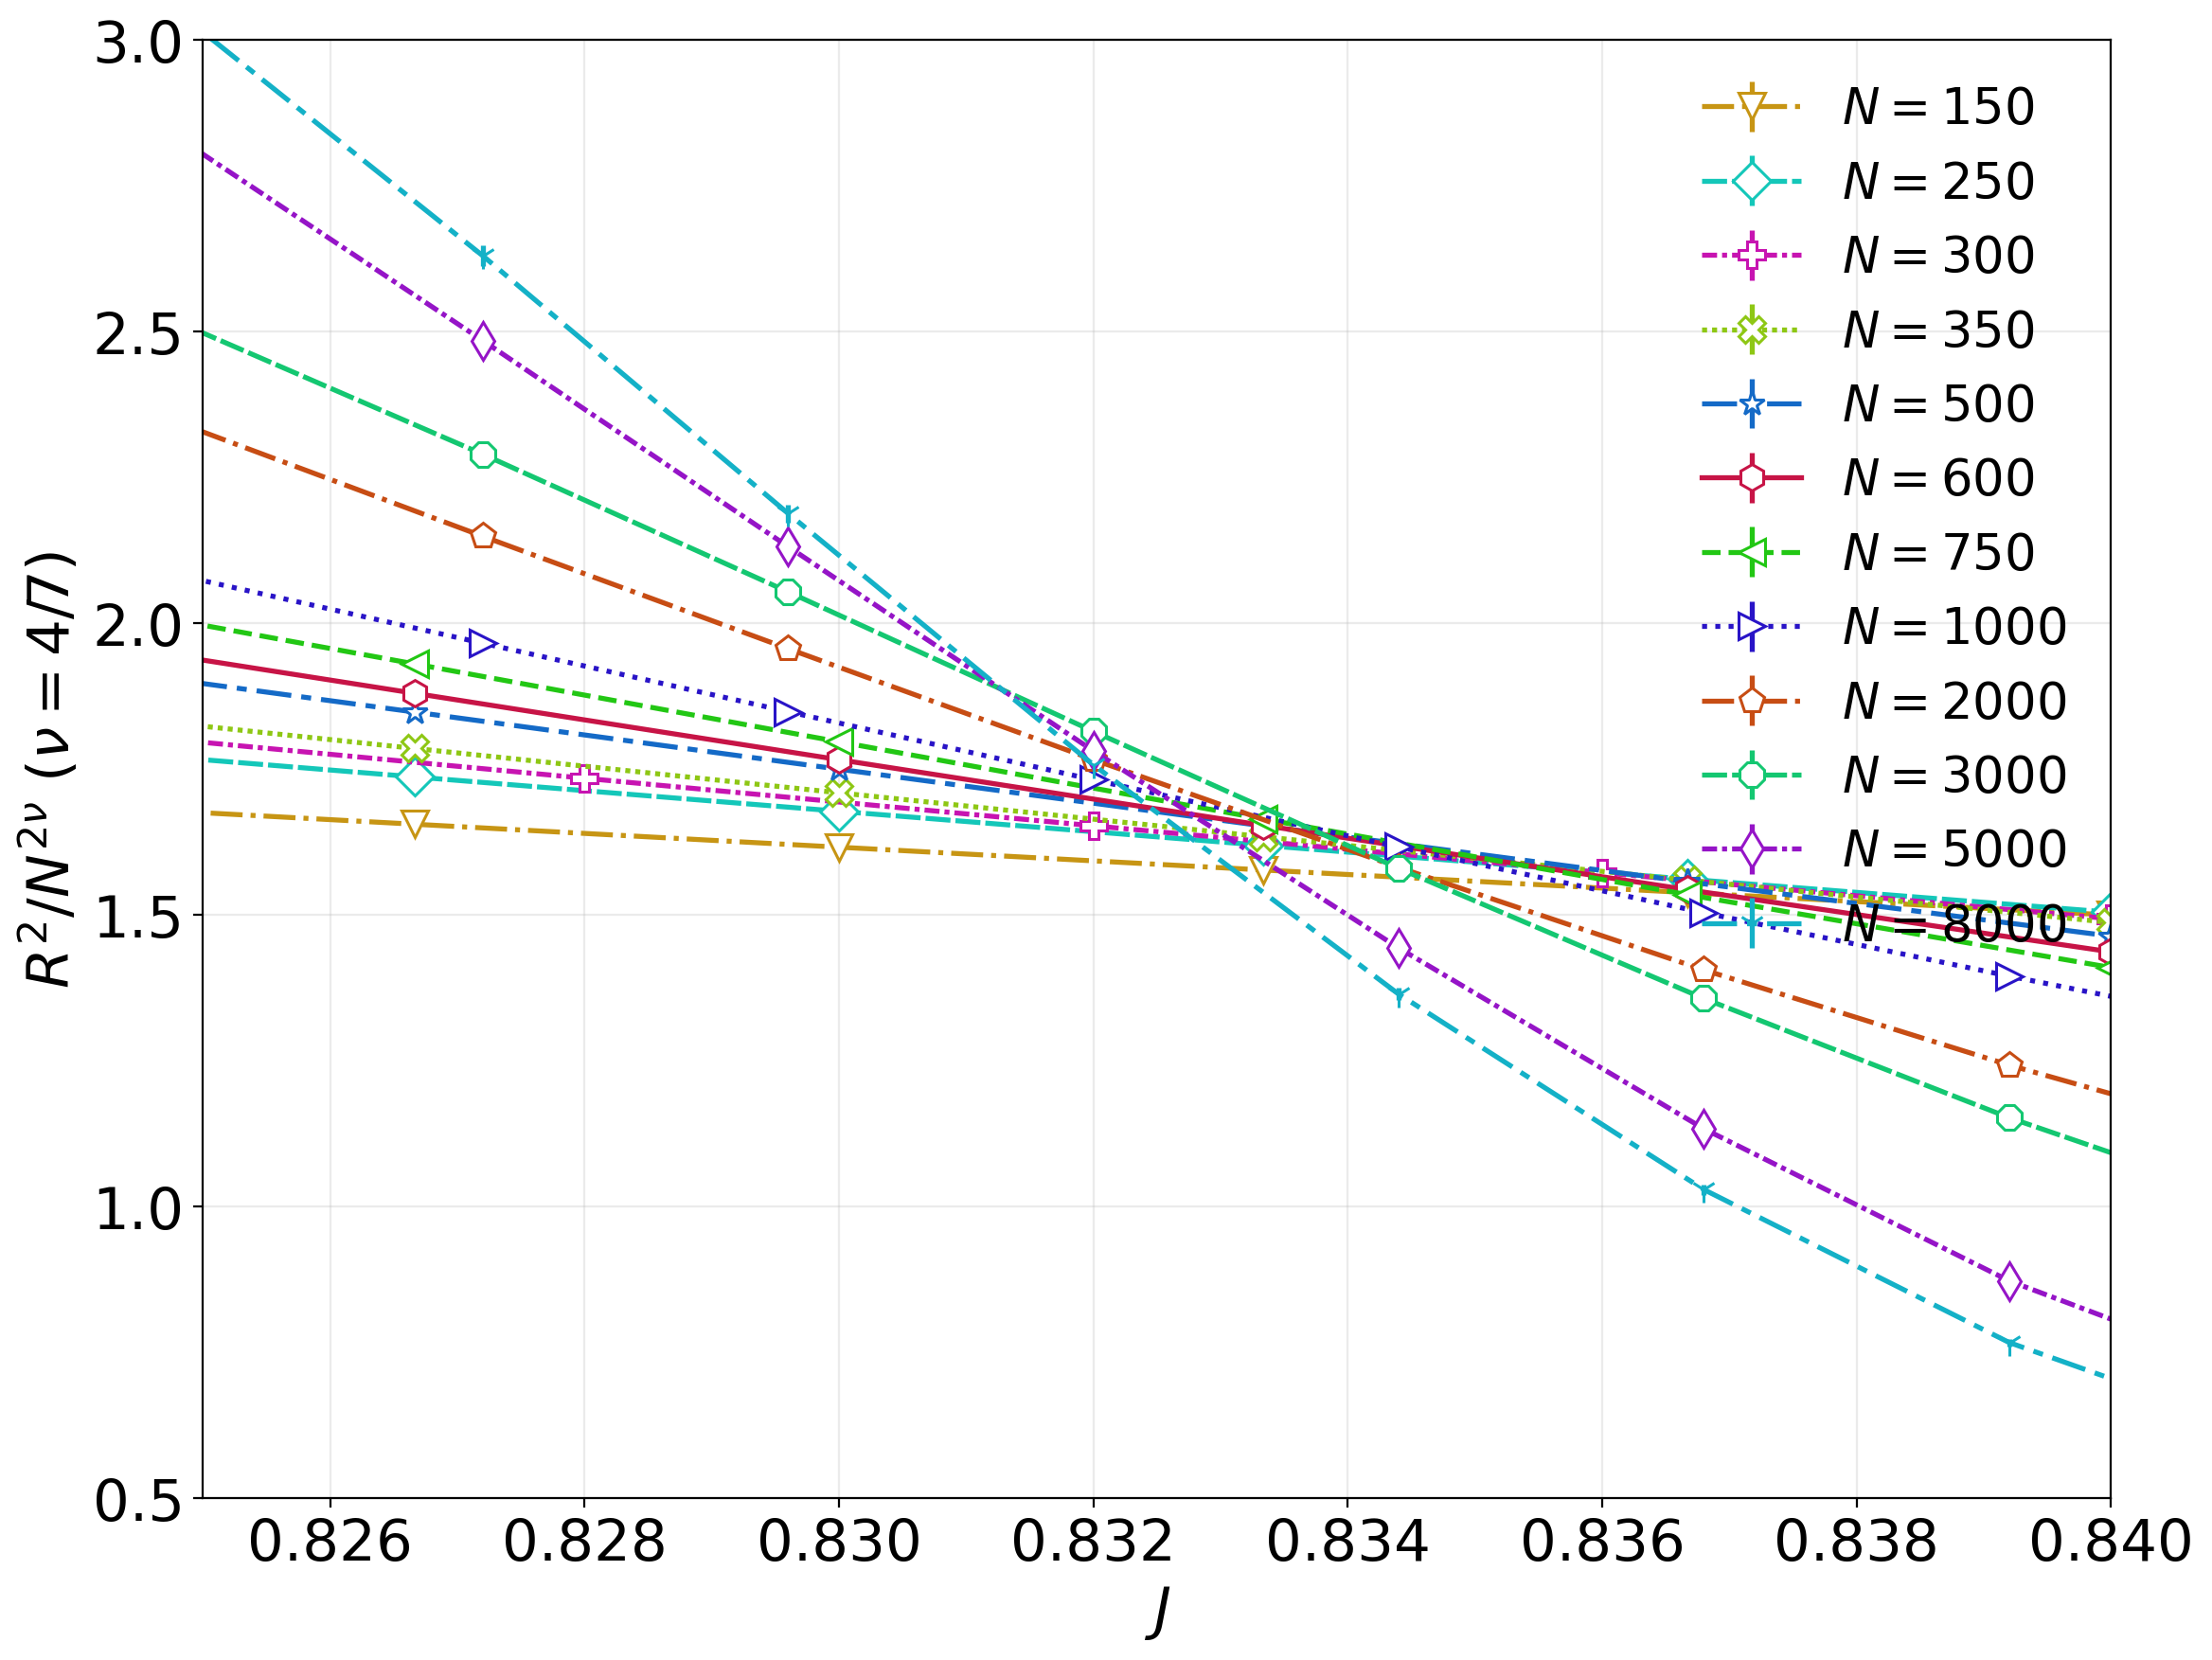
\includegraphics[width=\linewidth,height=0.58\textheight,keepaspectratio]{SI_ISing_2D_R2_scaled_nu057_reweight_zoomin.png}
    \column{0.50\textwidth}
    \[
      \widetilde R_N^2(J)=
      \frac{\langle R_N^2\rangle_J}{N^{2\nu_\Theta}},
      \qquad \nu_\Theta=\frac47.
    \]
    \[
      J_\times(N_1,N_2)=J_\infty+aN_{\mathrm{eff}}^{-\omega},
      \qquad N_{\mathrm{eff}}=\sqrt{N_1N_2}.
    \]
    \begin{itemize}
      \item Второй набор данных: обмен репликами в узком окне \(J\).
      \item Пересечения дают \(J_\Theta=0.8326(35)\).
      \item Магнитные пересечения дают \(J_{\mathrm{cr}}\simeq0.8348\).
      \item \(\phi_\Theta^{\mathrm{eff}}\simeq0.69\): сильные конечномерные поправки.
    \end{itemize}
  \end{columns}
\end{frame}

\begin{frame}{Изинг 2D: корреляция контактов и намагниченности}
  \scriptsize
  \[
    \rho_P(J)=
    \frac{\langle C|m|\rangle-\langle C\rangle\langle |m|\rangle}
    {\sqrt{\mathrm{Var}(C)\mathrm{Var}(|m|)}},
    \qquad
    \rho_S(J)=\rho_P(R_C,R_m).
  \]
  \begin{columns}[T,onlytextwidth]
    \column{0.50\textwidth}
      \centering
      \includegraphics[width=\linewidth,height=0.55\textheight,keepaspectratio]{SI_ISing_2D_pearson_reweight.png}
    \column{0.50\textwidth}
      \centering
      \includegraphics[width=\linewidth,height=0.55\textheight,keepaspectratio]{SI_ISing_2D_spearman_reweight.png}
  \end{columns}
  \small
  В изинговском случае рост контактной плотности статистически связан с ростом \(|m|\); это объясняет, почему \(J_\Theta\) и \(J_{\mathrm{cr}}\) практически совпадают.
\end{frame}

\begin{frame}{Изинг 2D: итоговая картина}
  \small
  \begin{columns}[T,onlytextwidth]
    \column{0.5\textwidth}
    \begin{block}{Совпадение критических областей}
      \[
        J_\Theta\simeq0.833,\qquad
        J_{\mathrm{cr}}\simeq0.834.
      \]
    \end{block}
    \begin{itemize}
      \item Коллапс цепи и магнитное упорядочение происходят вместе.
      \item Переход непрерывный в доступном диапазоне размеров.
      \item Геометрический показатель \(\nu_\Theta=4/7\) сохраняется.
    \end{itemize}
    \column{0.5\textwidth}
    \begin{block}{Механизм}
      Дискретное упорядочение Изинга хорошо конвертирует рост контактной плотности в магнитный выигрыш, поэтому геометрическая и магнитная перестройки синхронизируются.
    \end{block}
    \begin{block}{Численные признаки}
      \(R_N^2/N^{8/7}\) пересекается около \(0.833\); \(U_4^{(m)}\) пересекается около \(0.834\); распределения остаются одномодальными.
    \end{block}
  \end{columns}
\end{frame}

\section{XY-модель на БСП}

\begin{frame}{XY на БСП: постановка задачи}
  \small
  \[
    H(u,\theta)=-J\sum_{\langle i,j\rangle\in\E(u)}
    \cos(\theta_i-\theta_j).
  \]
  \begin{columns}[T,onlytextwidth]
    \column{0.5\textwidth}
    \begin{block}{Отличие от Изинга}
      У непрерывных спинов есть мягкие угловые флуктуации: рост числа контактов не обязан сразу давать жесткий ферромагнитный порядок.
    \end{block}
    \begin{block}{В 2D}
      Нужно отличать обычный магнитный переход от БКТ-подобной критической области.
    \end{block}
    \column{0.5\textwidth}
    \centering
    \includegraphics[width=0.62\linewidth]{state_glob_1.png}
    \vspace{0.3em}

    \scriptsize
    Цвет узлов кодирует углы \(\theta_i\).
  \end{columns}
  \source{Faizullina and Burovski, Phys. Rev. E 112, 024107 (2025).}
\end{frame}

\begin{frame}{XY 2D: структурный переход}
  \scriptsize
  \[
    \nu_\Theta=\frac47,\qquad
    J_\Theta\approx1.3634\pm0.005.
  \]
  \begin{columns}[T,onlytextwidth]
    \column{0.60\textwidth}
    \centering
    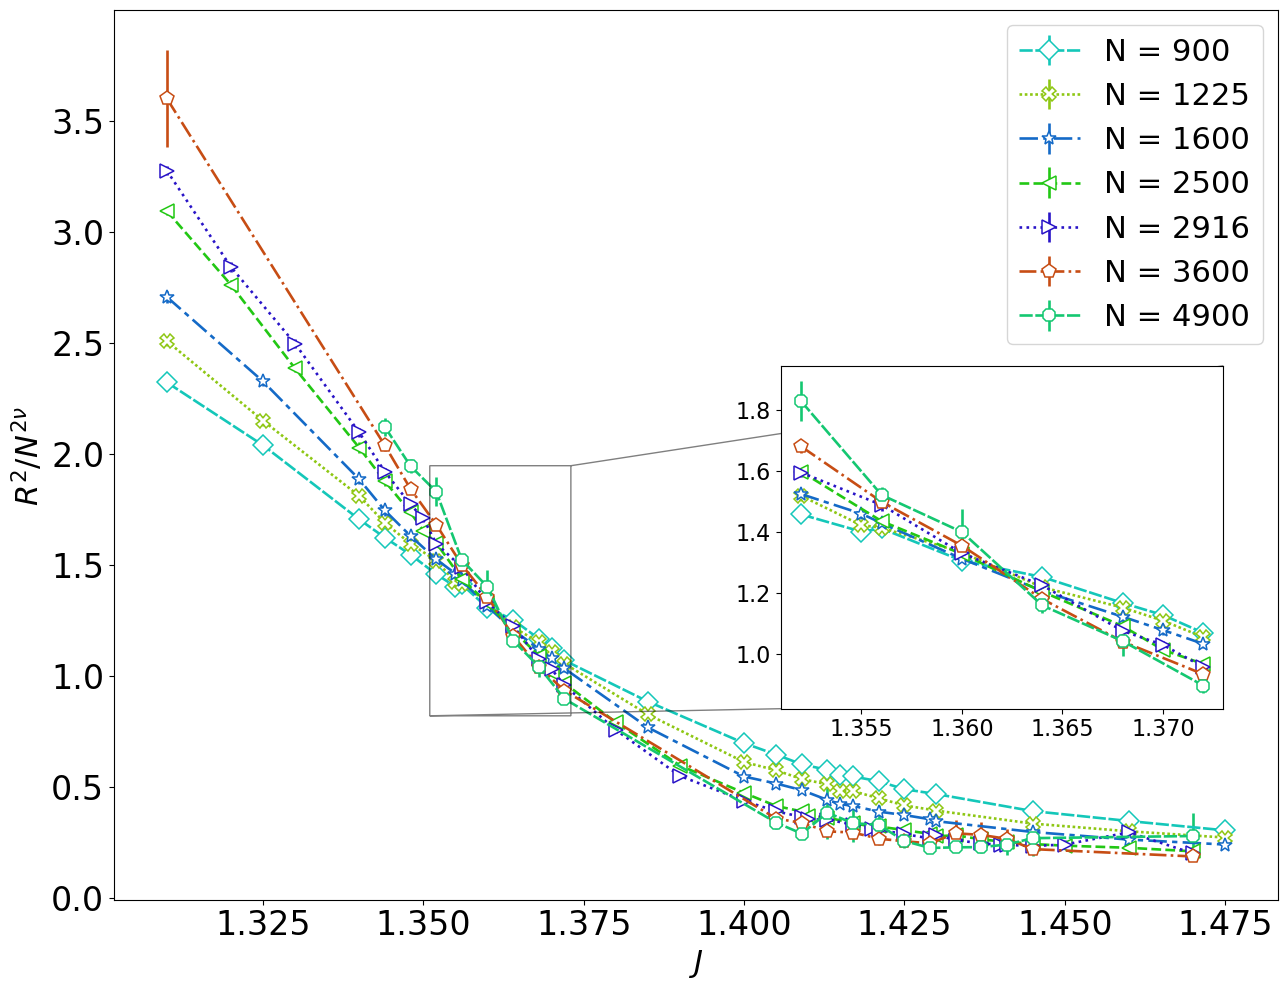
\includegraphics[width=\linewidth,height=0.62\textheight,keepaspectratio]{SI_XY_2D_r2_scale_long_fixed.png}
    \column{0.40\textwidth}
    \begin{itemize}
      \item Отмасштабированные радиусы сходятся в области \(J\simeq1.36\).
      \item Класс универсальности геометрии остается \(\Theta\)-подобным.
      \item Прямое моделирование показывает, что компактизация происходит раньше магнитной области.
    \end{itemize}
  \end{columns}
\end{frame}

\begin{frame}{XY 2D: примеры состояний при \(N=3600\)}
  \small
  \begin{columns}[T,onlytextwidth]
    \column{0.5\textwidth}
    \centering
    \includegraphics[width=0.88\linewidth,height=0.70\textheight,keepaspectratio]{xy2d_state_L3600_coil_J1p32.png}

    \scriptsize
    Развернутое состояние: \(J=1.320<J_\Theta\).

    \column{0.5\textwidth}
    \centering
    \includegraphics[width=0.88\linewidth,height=0.70\textheight,keepaspectratio]{xy2d_state_L3600_globule_J1p404.png}

    \scriptsize
    Свернутое состояние: \(J=1.404>J_\Theta\).
  \end{columns}

\end{frame}

\begin{frame}{XY 2D: магнитная область отделена от \(\Theta\)-точки}
  \small
  \begin{columns}[T,onlytextwidth]
    \column{0.53\textwidth}
    \centering
    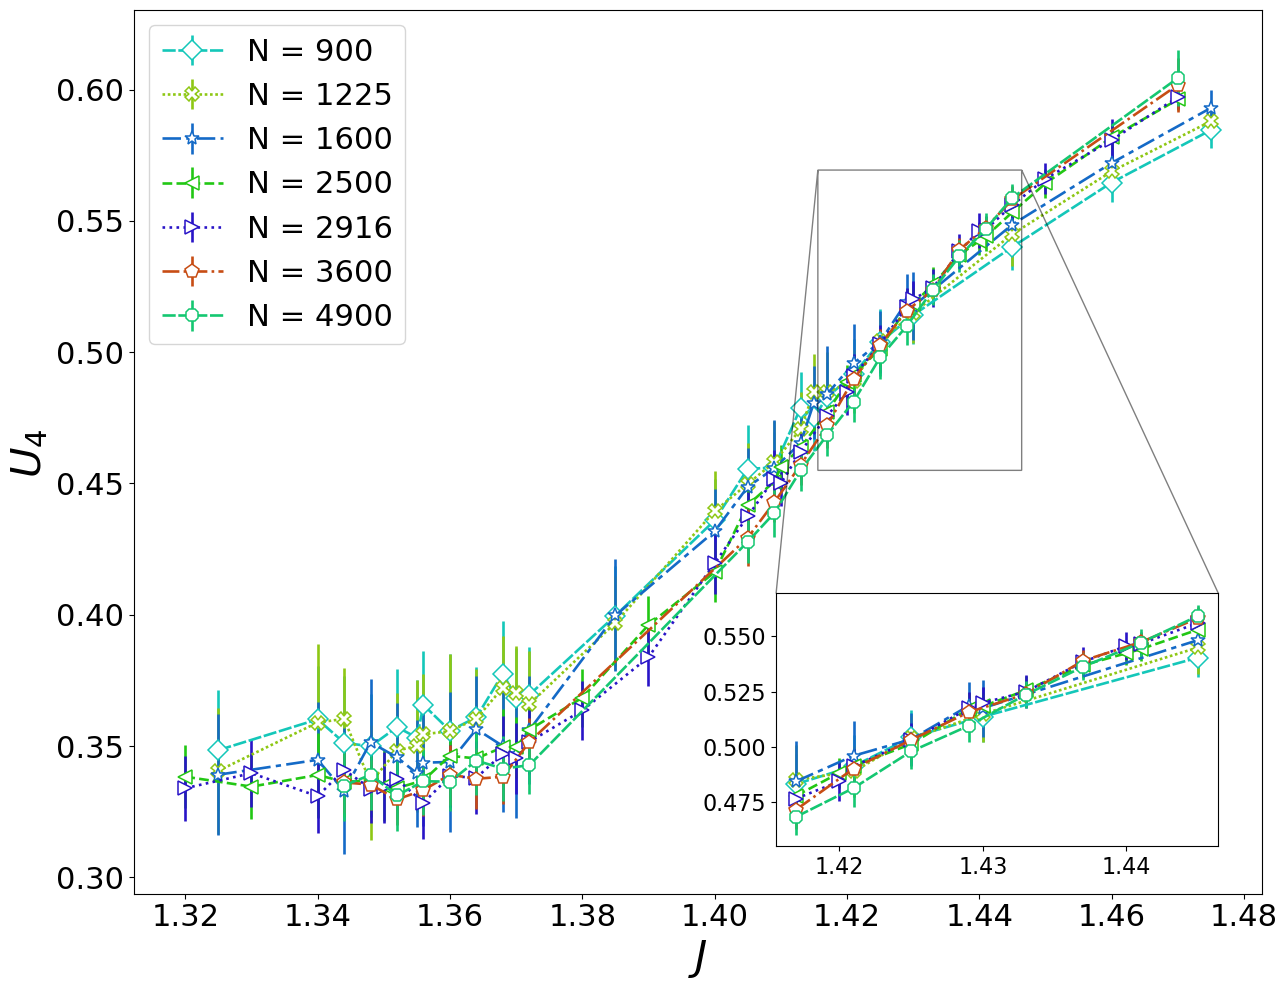
\includegraphics[width=\linewidth]{SI_XY_2D_U4_long_fixed.png}
    \column{0.47\textwidth}
    \begin{block}{По кумулянтам Биндера}
      \[
        U_4=1-\frac{\langle m^4\rangle}{3\langle m^2\rangle^2},
        \qquad
        J_{\mathrm{cr}}\approx1.435\pm0.008
      \]
      по прямому моделированию.
    \end{block}
    \[
      J_\Theta\simeq1.36 < J_{\mathrm{cr}}.
    \]
  \end{columns}
\end{frame}

\begin{frame}{XY 2D: сырая намагниченность}
  \small
  \[
    H(u,\theta)=-J\sum_{\langle i,j\rangle\in\E(u)}
    \cos(\theta_i-\theta_j),
    \qquad
    m^2=M_x^2+M_y^2.
  \]
  \begin{columns}[T,onlytextwidth]
    \column{0.64\textwidth}
      \centering
      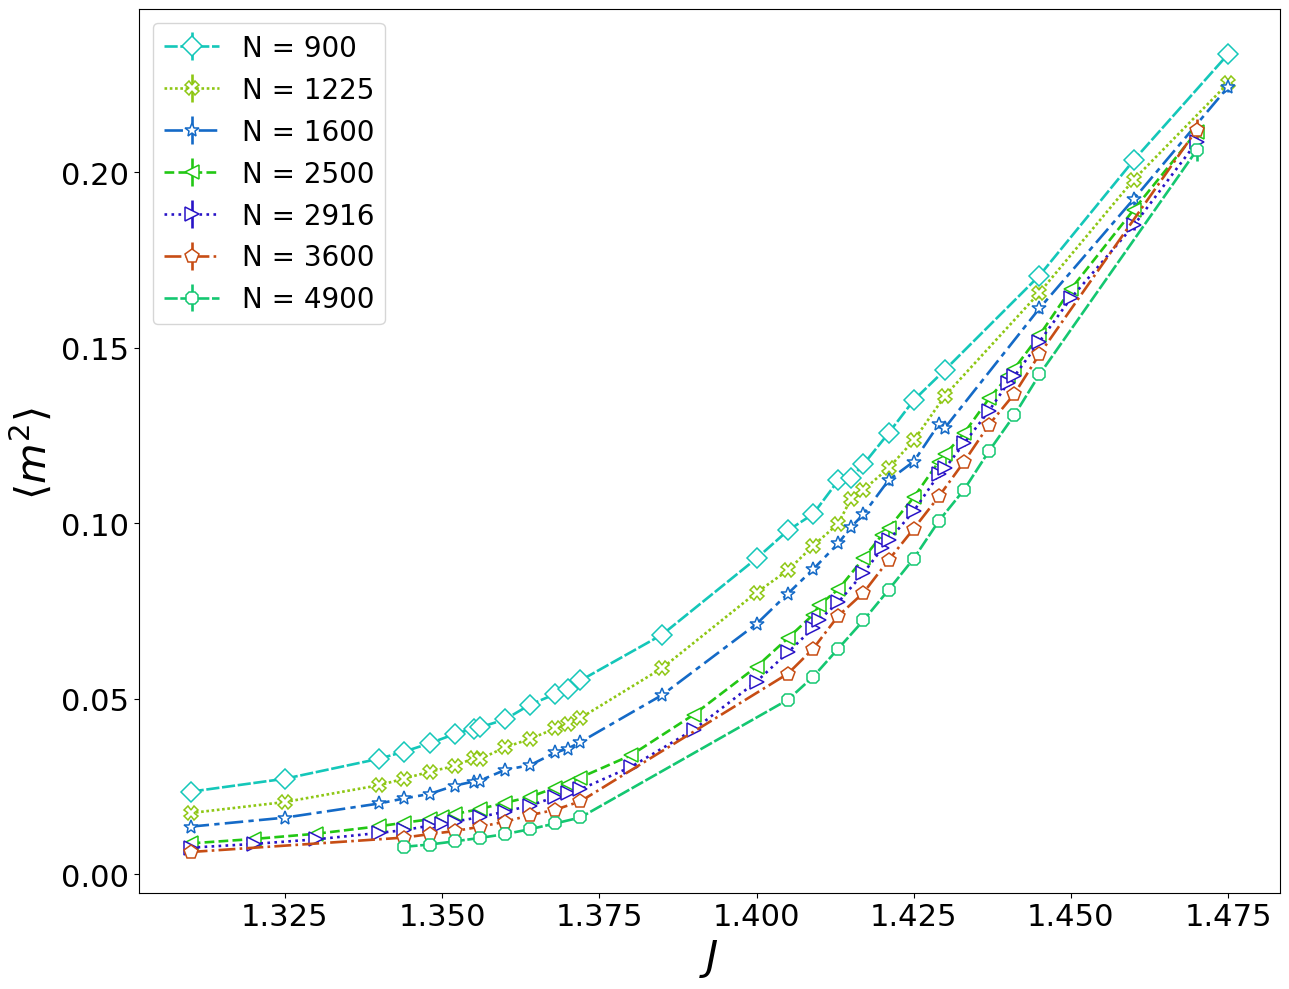
\includegraphics[width=\linewidth,height=0.62\textheight,keepaspectratio]{SI_XY_2D_m2_long_fixed.png}
    \column{0.36\textwidth}
      \begin{itemize}
        \item \(\langle m^2\rangle\) растет плавно, без скачка.
        \item Размерная зависимость сильная: в 2D обычный дальний порядок не является правильной картиной.
        \item Магнитная область начинается правее \(J_\Theta\simeq1.36\).
      \end{itemize}
  \end{columns}
\end{frame}

\begin{frame}{XY 2D: масштабированная намагниченность}
  \scriptsize
  В БКТ-подобной области ожидается алгебраическое убывание корреляций; для конечной системы это проявляется как степенная размерная зависимость намагниченности:
  \[
    \langle m^2\rangle \sim N^{-\eta_m(J)},\qquad
    \langle m^2\rangle N^{\eta_m}\approx \text{const}.
  \]
  \begin{columns}[T,onlytextwidth]
    \column{0.64\textwidth}
      \centering
      \includegraphics[width=\linewidth,height=0.45\textheight,keepaspectratio]{SI_XY_2D_m2scaled_reweight.png}
    \column{0.36\textwidth}
      \begin{itemize}
        \item Масштабирование с эффективным показателем порядка \(1/4\) собирает кривые в области \(J\simeq1.42\).
        \item Это не отдельное доказательство БКТ-перехода, а согласованный конечномерный признак.
        \item Та же область видна по \(U_4\) и корреляционным функциям.
      \end{itemize}
  \end{columns}
\end{frame}

\begin{frame}{XY 2D: корреляционные функции}
  \scriptsize
  \[
    G(r)=
    \left\langle
    \frac{1}{n_u(r)}
    \sum_{(i,j)\in\mathcal P_u(r)}
    \cos(\theta_i-\theta_j)
    \right\rangle .
  \]
  \begin{columns}[T,onlytextwidth]
    \column{0.48\textwidth}
    \centering
    \includegraphics[width=\linewidth,height=0.38\textheight,keepaspectratio]{eta_vs_J.png}
    \[
      G(r)\sim r^{-\eta(J)},\qquad
      \eta(J_{\mathrm{BKT}})=\frac14
    \]
    дает \(J_{\eta=1/4}^{\mathrm{eff}}\simeq1.42\).
    \column{0.52\textwidth}
    \centering
    \includegraphics[width=\linewidth,height=0.46\textheight,keepaspectratio]{corrs_vs_r_ru1.png}
  \end{columns}
  \scriptsize
  Показатель корреляционной функции, \(U_4\) и масштабированная намагниченность указывают на одну область \(J\simeq1.42\).
\end{frame}

\begin{frame}{XY 2D: состояние в магнитной области}
  \centering
  \includegraphics[width=0.88\paperwidth,height=0.70\paperheight,keepaspectratio]{xy2d_state_bkt_user_attachment.png}

  \vspace{0.2em}
  \scriptsize
  Пример конфигурации около \(J\simeq1.426\): цепь уже компактна, но угловая структура остается мягкой и неоднородной.
\end{frame}

\begin{frame}{XY 2D: распределение энергии}
  \small
  \[
    e=H/N,\qquad
    J_\Theta\simeq1.36,\quad J_{\mathrm{cr}}\simeq1.42\text{--}1.44 .
  \]
  \centering
  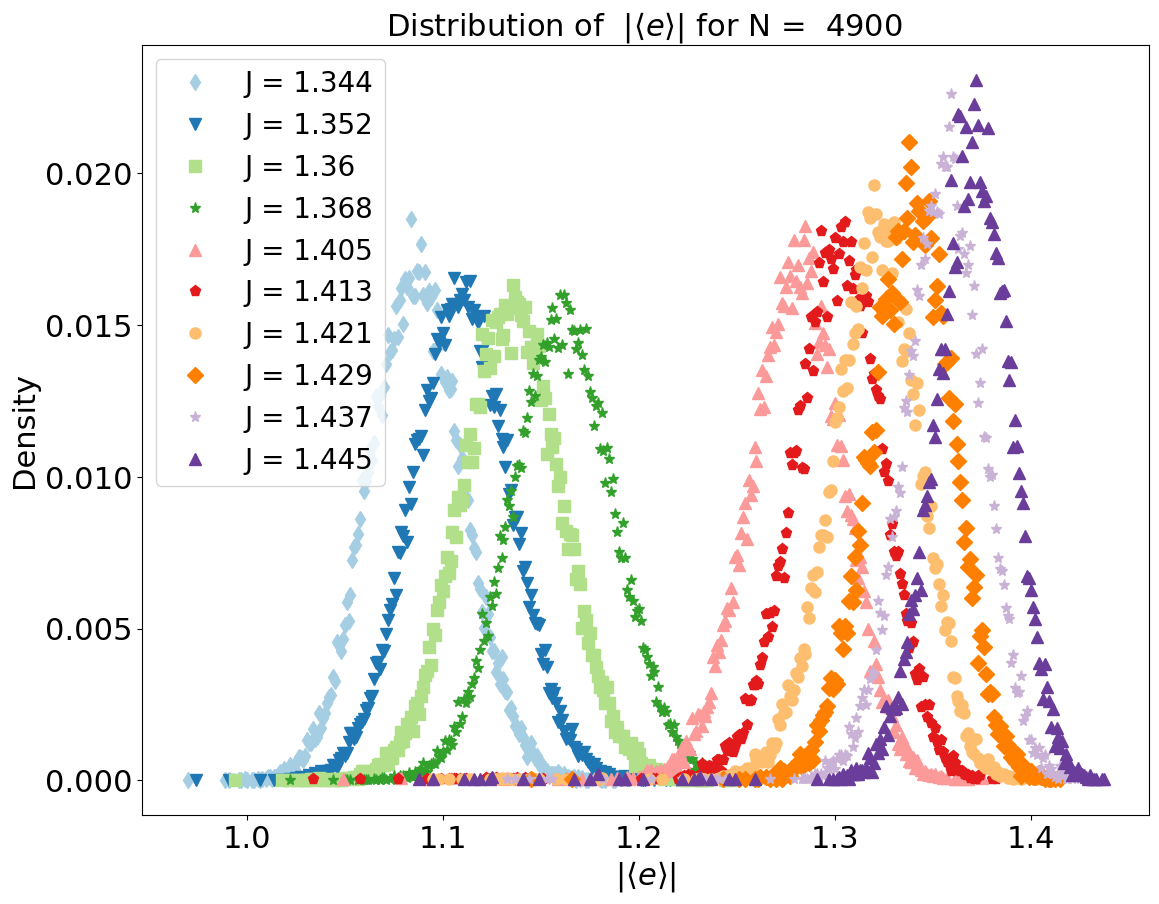
\includegraphics[width=0.72\linewidth,height=0.66\textheight,keepaspectratio]{SI_XY_2D_distr_e1_4900.png}

  \vspace{0.2em}
  \scriptsize
  \(N=4900\). Пики смещаются с \(J\), но не распадаются на устойчивую двухфазную структуру.
\end{frame}

\begin{frame}{XY 2D: триптих распределений}
  \centering
  \includegraphics[width=0.98\textwidth,height=0.78\textheight,keepaspectratio]{triptych_L_XY_SI_2D_4900.png}

  {\scriptsize Слева направо: \(P(e)\), \(P(|m|)\), \(P(C/N)\); признаки сосуществования фаз в двумерной XY-модели не наблюдаются.}
\end{frame}

\begin{frame}{XY 2D: анализ перевзвешенных данных}
  \scriptsize
  \begin{columns}[T,onlytextwidth]
    \column{0.50\textwidth}
    \centering
    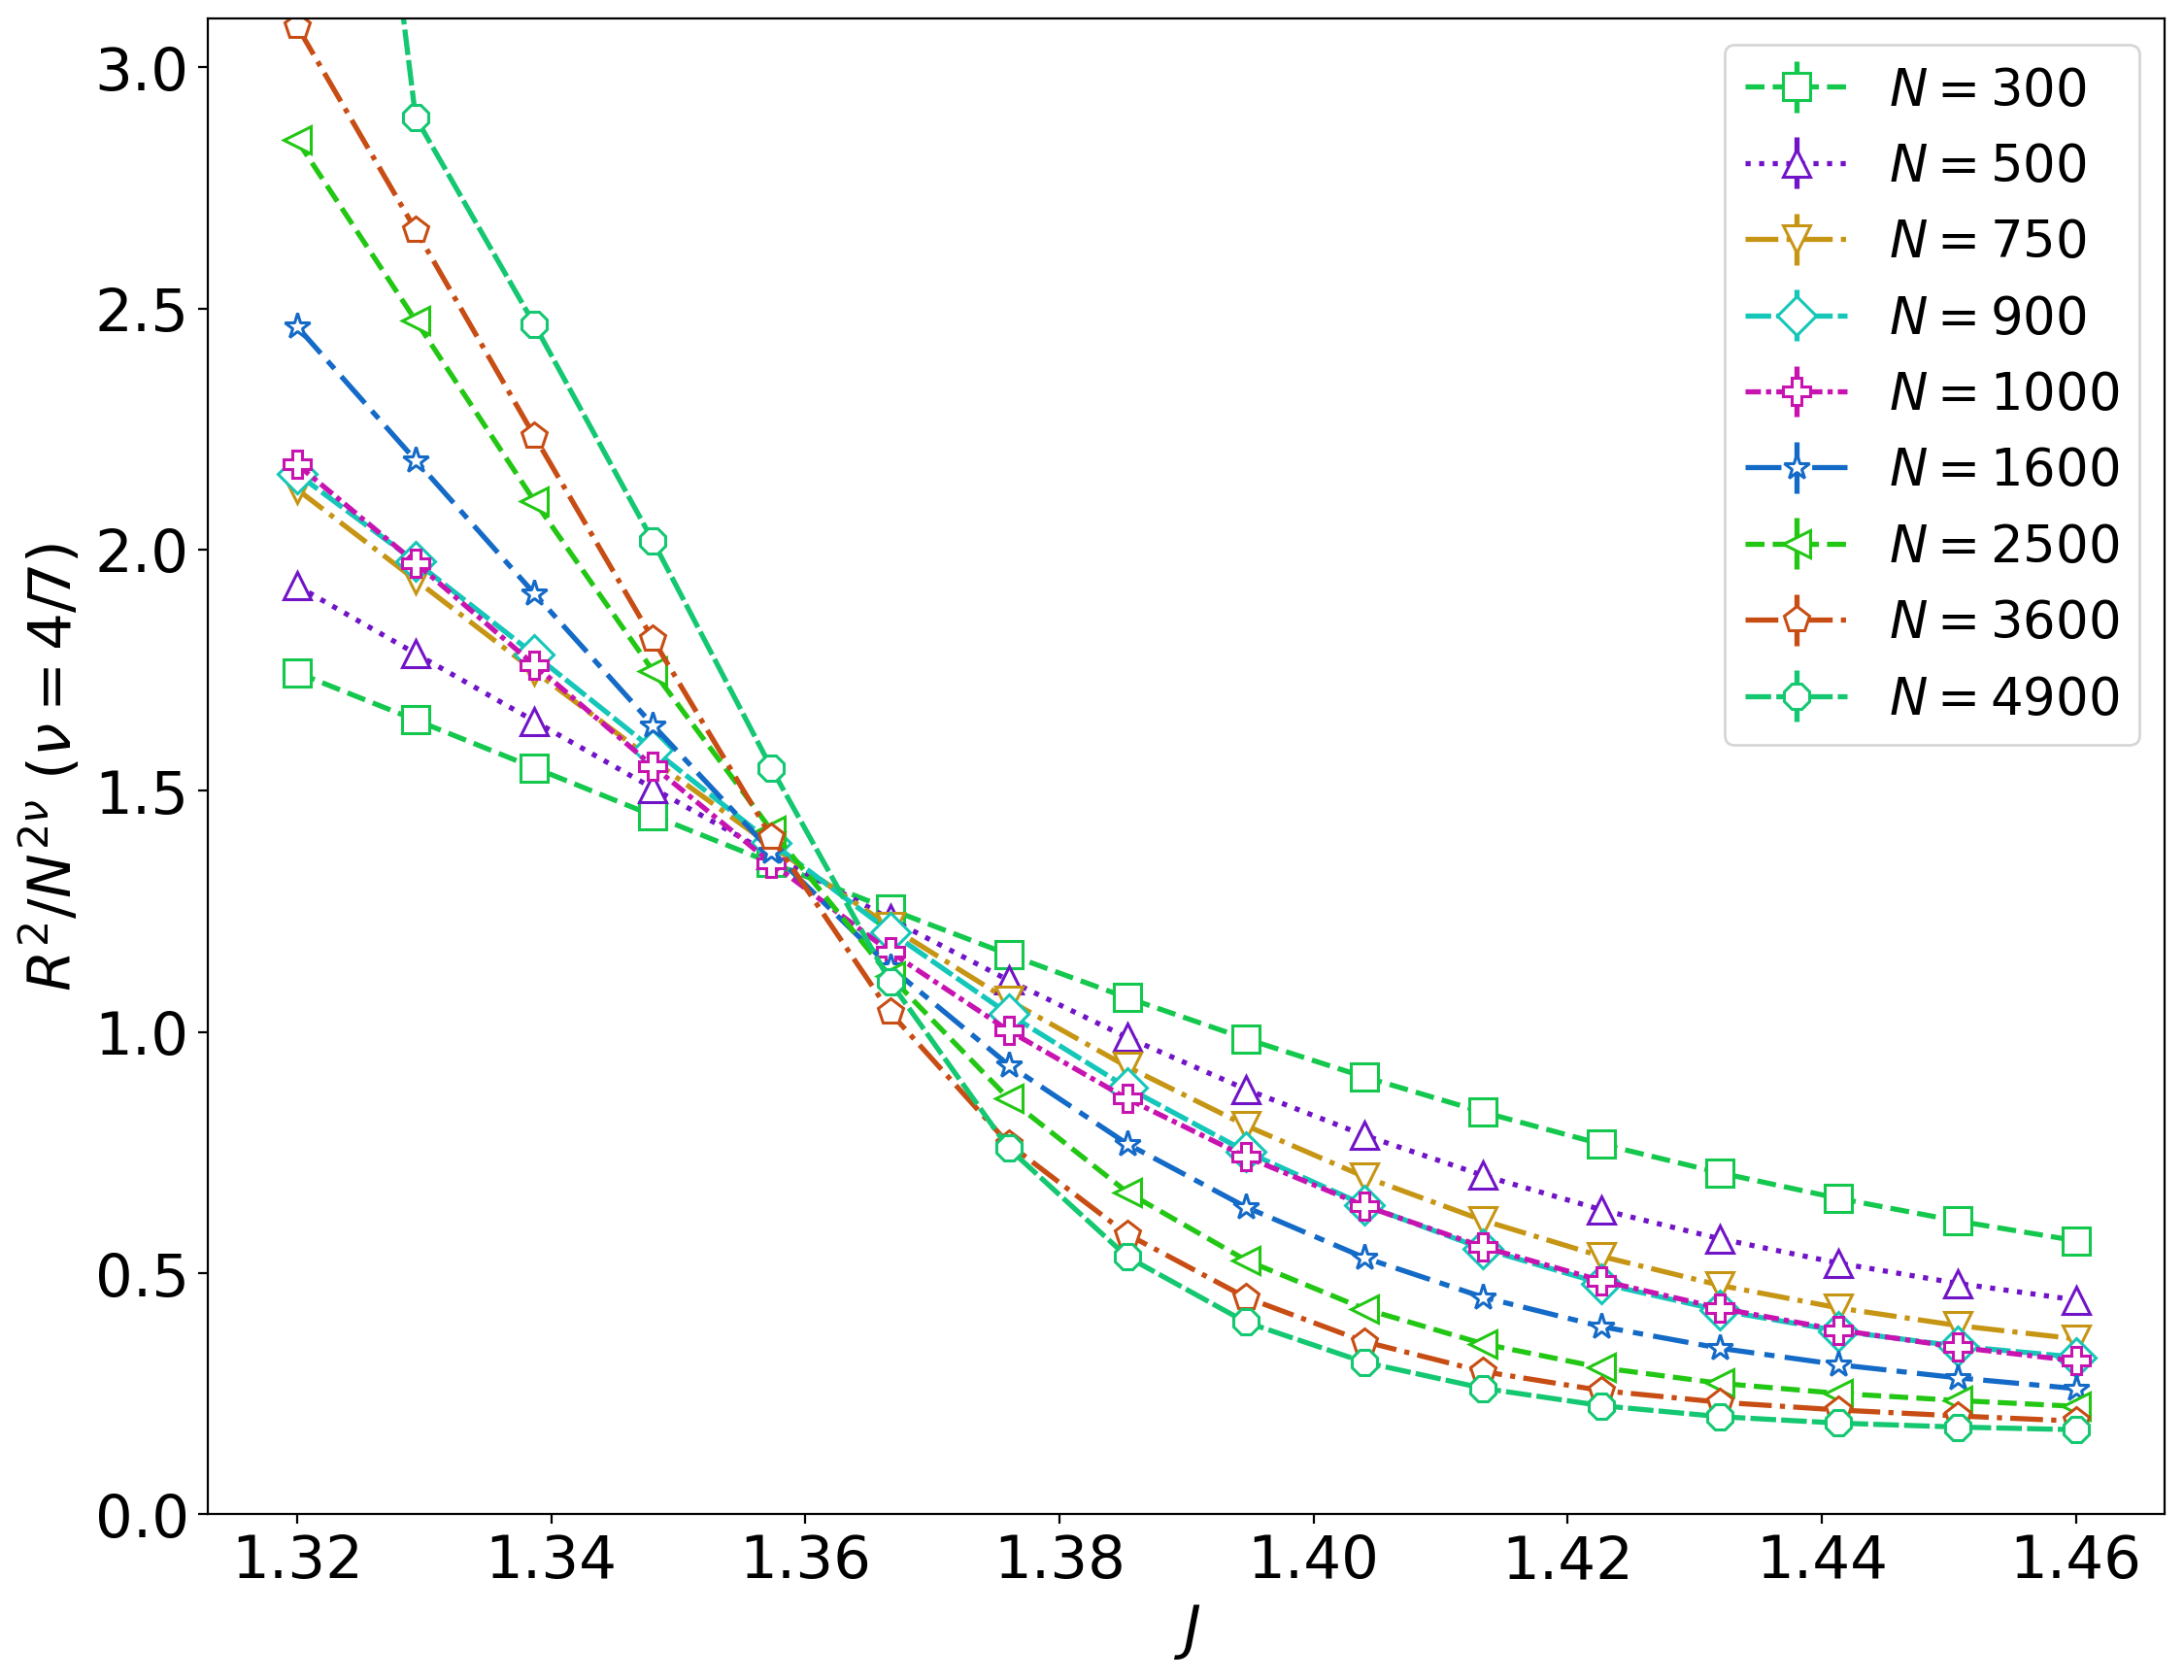
\includegraphics[width=\linewidth,height=0.35\textheight,keepaspectratio]{SI_XY_2D_R2_scaled_nu057_reweight.png}
    \[
      J_\Theta\simeq1.36\text{--}1.37,\qquad
      \phi_\Theta^{\mathrm{eff}}\simeq0.52.
    \]
    \column{0.50\textwidth}
    \[
      \widetilde R_N^2(J)=
      \frac{\langle R_N^2\rangle_J}{N^{2\nu_\Theta}},
      \qquad \nu_\Theta=\frac47.
    \]
    \[
      \langle O\rangle_J=
      \frac{\sum_Q \overline O(Q)\Omega(Q)e^{JQ}}
      {\sum_Q \Omega(Q)e^{JQ}}.
    \]
    \begin{itemize}
      \item Перевзвешивание уточняет структурную область, а не создает новый физический критерий.
      \item Оценка \(J_\Theta\) остается левее магнитной области.
      \item Эффективный \(\phi_\Theta\) завышен относительно \(3/7\), что указывает на конечномерные поправки.
    \end{itemize}
  \end{columns}
\end{frame}

\begin{frame}{XY 2D: корреляция контактов и намагниченности}
  \scriptsize
  \[
    \rho_P(J)=
    \frac{\langle C|m|\rangle-\langle C\rangle\langle |m|\rangle}
    {\sqrt{\mathrm{Var}(C)\mathrm{Var}(|m|)}},
    \qquad
    \rho_S(J)=\rho_P(R_C,R_m).
  \]
  \begin{columns}[T,onlytextwidth]
    \column{0.50\textwidth}
      \centering
      \includegraphics[width=\linewidth,height=0.55\textheight,keepaspectratio]{SI_XY_2D_pearson_reweight.png}
    \column{0.50\textwidth}
      \centering
      \includegraphics[width=\linewidth,height=0.55\textheight,keepaspectratio]{SI_XY_2D_spearman_reweight.png}
  \end{columns}
  \small
  В 2D XY корреляции между \(C\) и \(|m|\) выражены слабее и не дают синхронизации \(J_\Theta\) с магнитной областью.
\end{frame}

\begin{frame}{XY 3D: структурная перестройка}
  \scriptsize
  \[
    \nu_\Theta=\frac12,\qquad
    J_\Theta\approx0.876(5)
  \]
  по прямому анализу масштабированных радиусов.
  \begin{columns}[T,onlytextwidth]
    \column{0.60\textwidth}
    \centering
    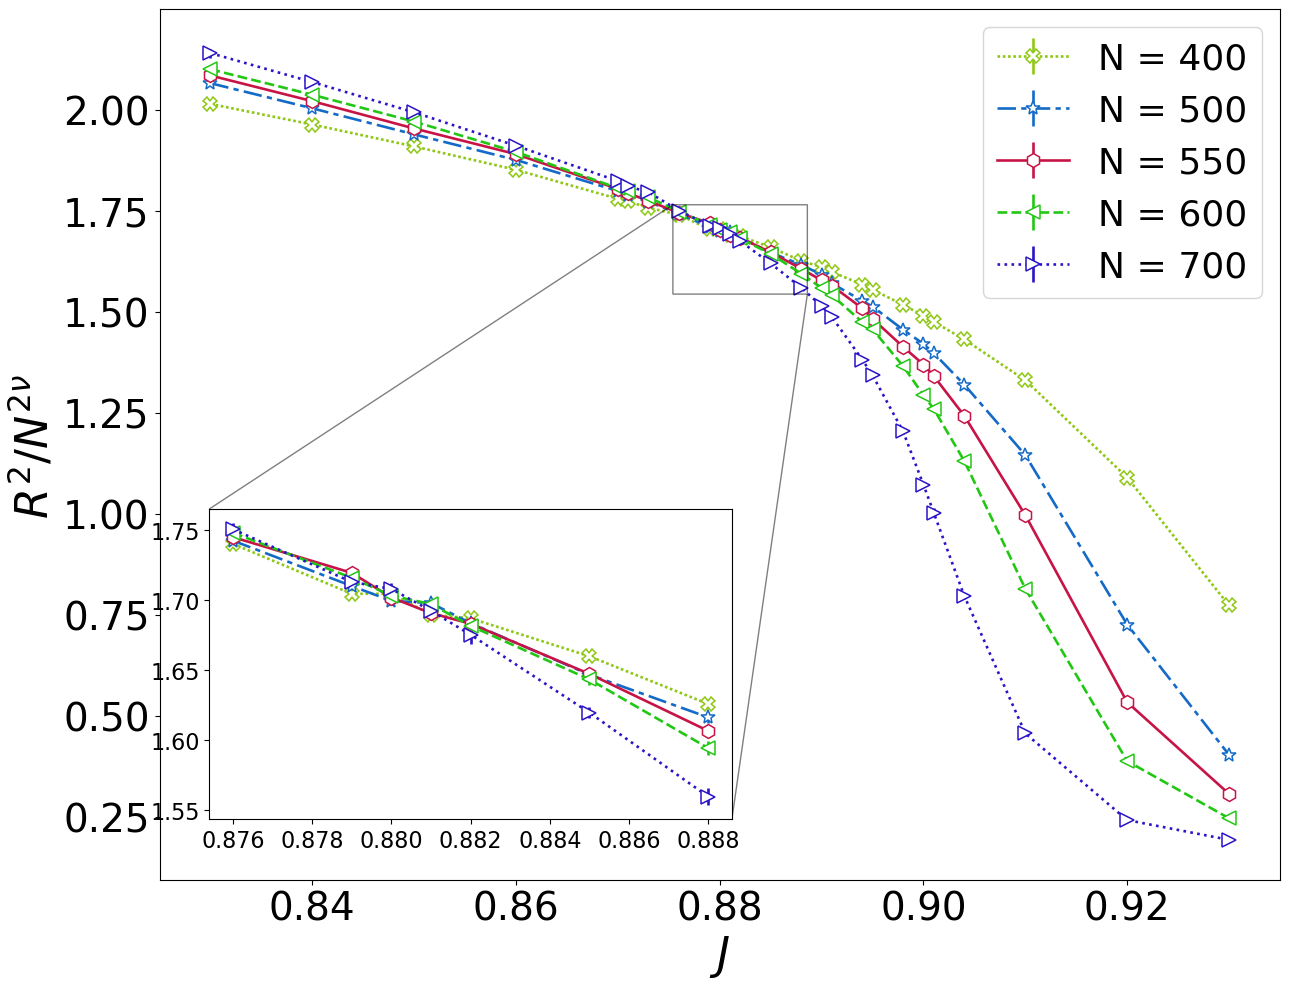
\includegraphics[width=\linewidth,height=0.62\textheight,keepaspectratio]{SI_XY_3D_r2_long_scale_fixed.png}
    \column{0.40\textwidth}
    \begin{itemize}
      \item Масштабированные радиусы дают область \(J\simeq0.87\).
      \item Геометрический показатель соответствует \(\Theta\)-полимеру в 3D.
      \item О порядке перехода судим по распределениям и кумулянтам.
    \end{itemize}
  \end{columns}
\end{frame}

\begin{frame}{XY 3D: контакты показывают резкую перестройку}
  \small
  \[
    U_4^{(C,\mathrm{cent})}
    =
    1-
    \frac{\langle (C-\langle C\rangle)^4\rangle}
    {3\langle (C-\langle C\rangle)^2\rangle^2}.
  \]
  \begin{columns}[T,onlytextwidth]
    \column{0.52\textwidth}
    \centering
    \includegraphics[width=\linewidth,height=0.46\textheight,keepaspectratio]{binder_contacts_centered.png}
    \column{0.48\textwidth}
    \centering
    \includegraphics[width=\linewidth,height=0.46\textheight,keepaspectratio]{XY_contacts_binder_extrema_extrapolation_ru.png}
  \end{columns}
  \scriptsize
  Отрицательный минимум углубляется с ростом \(N\): распределение числа контактов становится негауссовым и указывает на сосуществование развернутых и компактных конформаций.
\end{frame}

\begin{frame}{XY 3D: магнитный переход с признаками первого рода}
  \scriptsize
  \begin{columns}[T,onlytextwidth]
    \column{0.58\textwidth}
    \centering
    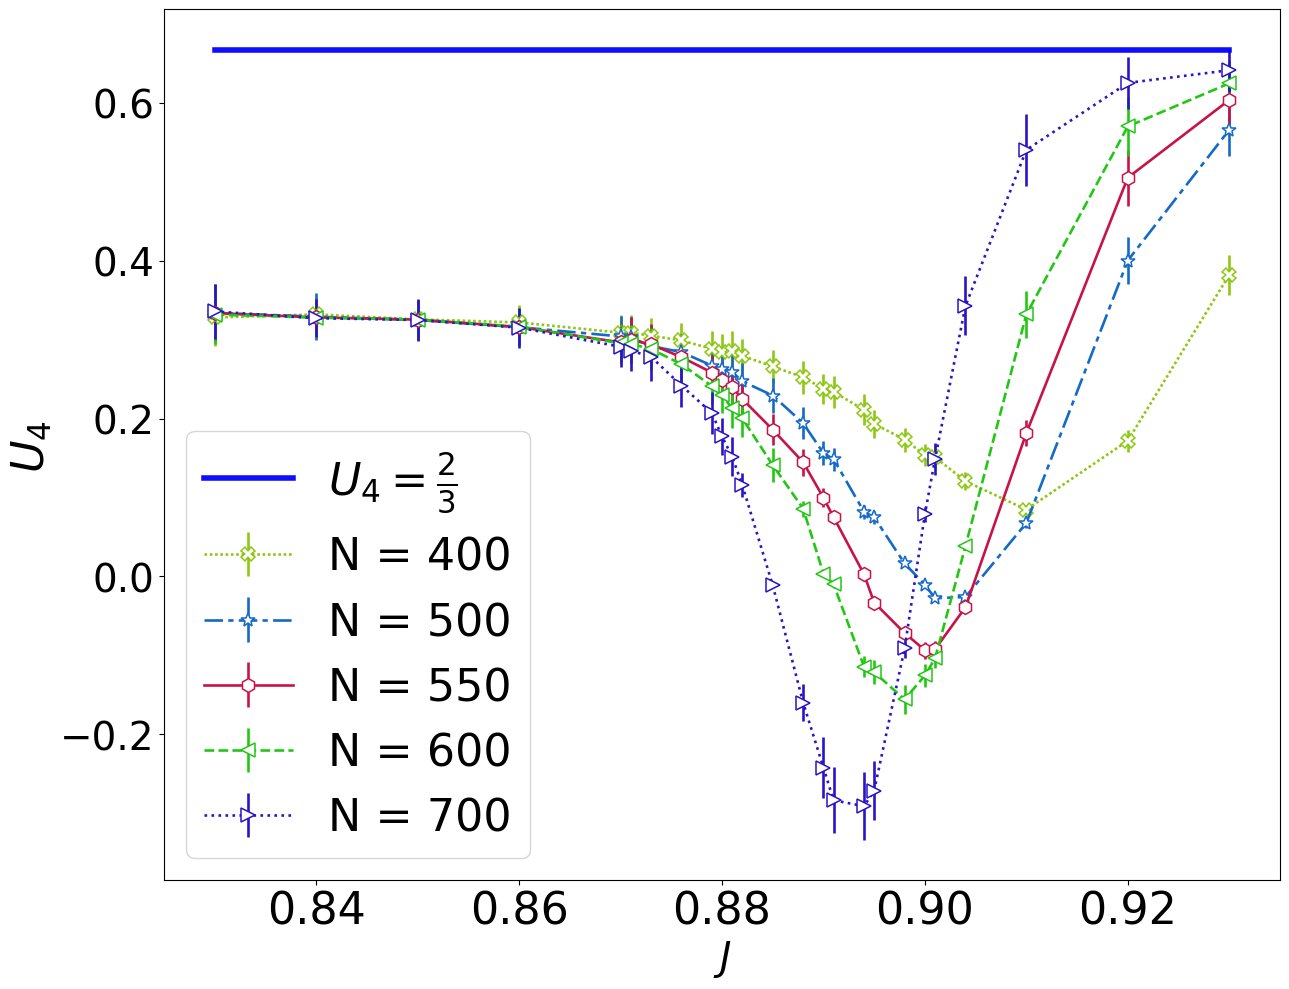
\includegraphics[width=\linewidth,height=0.64\textheight,keepaspectratio]{SI_XY_3D_U4_long_fixed.png}
    \column{0.42\textwidth}
    \[
      U_4^{(m)}=
      1-\frac{\langle m^4\rangle}{3\langle m^2\rangle^2}.
    \]
    \begin{itemize}
      \item В области \(J\simeq0.87\)--\(0.91\) появляется отрицательный минимум \(U_4^{(m)}\).
      \item Минимум углубляется при росте \(N\).
      \item Вместе с бимодальными распределениями это численный признак первого рода.
    \end{itemize}
  \end{columns}
\end{frame}

\begin{frame}{XY 3D: распределение энергии}
  \small
  \[
    e=H/N,\qquad
    J\simeq0.898\text{--}0.92 .
  \]
  \centering
  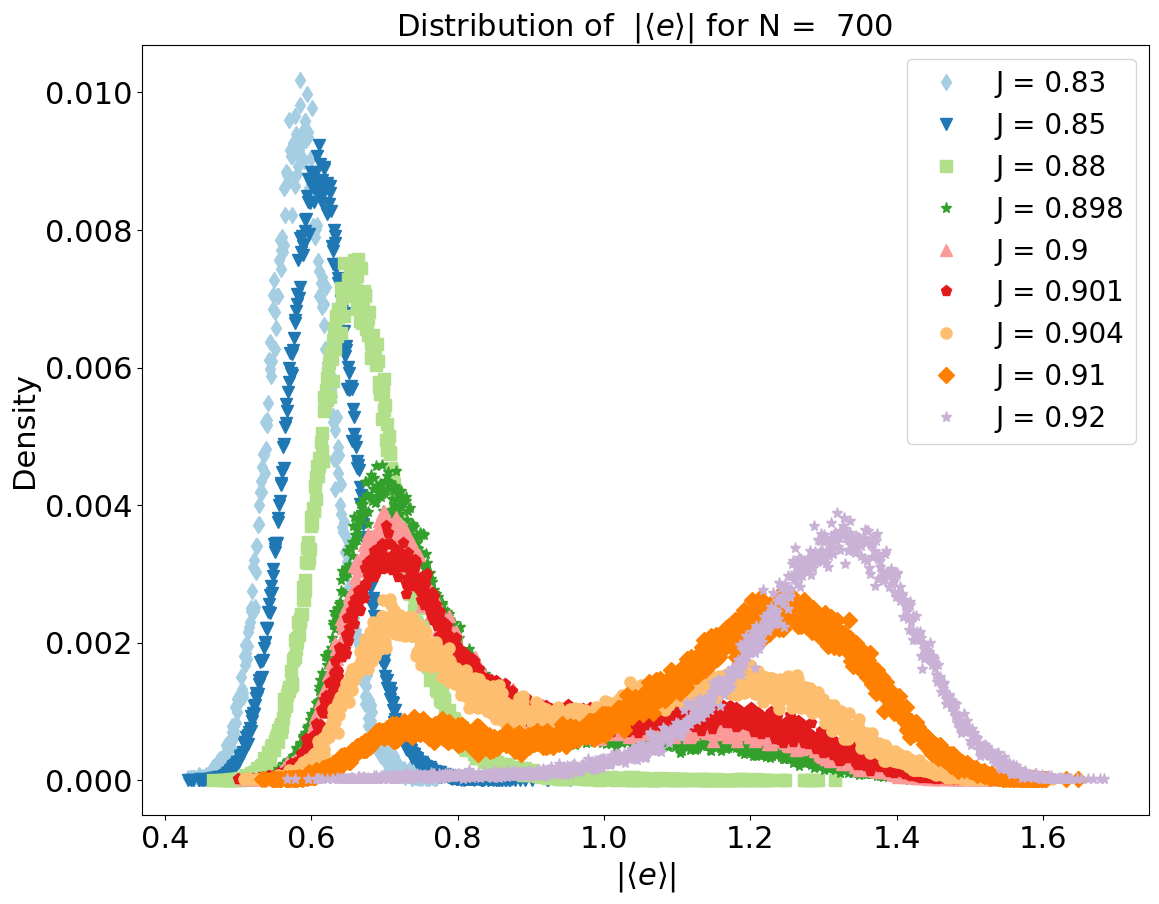
\includegraphics[width=0.72\linewidth,height=0.66\textheight,keepaspectratio]{SI_XY_3D_distr_e1_700.png}

  \vspace{0.2em}
  \scriptsize
  \(N=700\). Бимодальность возникает в той же области, где \(U_4^{(m)}\) имеет отрицательный минимум.
\end{frame}

\begin{frame}{XY 3D: триптих распределений}
  \centering
  \includegraphics[width=0.98\textwidth,height=0.78\textheight,keepaspectratio]{triptych_L_XY_SI_3D_700.png}

  {\scriptsize \(N=700\). Слева направо: \(P(e)\), \(P(|m|)\), \(P(C/N)\); два типа состояний видны сразу в трех наблюдаемых.}
\end{frame}

\begin{frame}{XY 3D: анализ перевзвешенных данных}
  \scriptsize
  \begin{columns}[T,onlytextwidth]
    \column{0.50\textwidth}
    \centering
    \includegraphics[width=\linewidth,height=0.52\textheight,keepaspectratio]{SI_XY_3D_R2_scaled_nu05_reweight_zoomin.png}
    \[
      J_\Theta\simeq0.87,\qquad \nu_\Theta=\frac12.
    \]
    \column{0.50\textwidth}
    \centering
    \includegraphics[width=\linewidth,height=0.52\textheight,keepaspectratio]{SI_XY_3D_binder_u3_reweight.png}
  \end{columns}
  Перевзвешивание уточняет положение псевдокритических точек; отрицательные минимумы кумулянтов сохраняются и согласуются с распределениями.
\end{frame}

\begin{frame}{XY 3D: корреляция контактов и намагниченности}
  \scriptsize
  \[
    \rho_P(J)=
    \frac{\langle C|m|\rangle-\langle C\rangle\langle |m|\rangle}
    {\sqrt{\mathrm{Var}(C)\mathrm{Var}(|m|)}},
    \qquad
    \rho_S(J)=\rho_P(R_C,R_m).
  \]
  \begin{columns}[T,onlytextwidth]
    \column{0.50\textwidth}
      \centering
      \includegraphics[width=\linewidth,height=0.55\textheight,keepaspectratio]{SI_XY_3D_pearson_reweight.png}
    \column{0.50\textwidth}
      \centering
      \includegraphics[width=\linewidth,height=0.55\textheight,keepaspectratio]{SI_XY_3D_spearman_reweight.png}
  \end{columns}
  \small
  В 3D рост \(C\) и \(|m|\) становится резко согласованным около \(J\simeq0.89\)--\(0.91\). Это и есть отличие от 2D XY: геометрия и магнитный порядок сцепляются.
\end{frame}

\begin{frame}{2D против 3D в XY-модели}
  \scriptsize
  \begin{tabularx}{\textwidth}{@{}>{\raggedright\arraybackslash}p{0.20\textwidth}>{\raggedright\arraybackslash}p{0.36\textwidth}>{\raggedright\arraybackslash}X@{}}
    \toprule
    Свойство & 2D квадратная решетка & 3D кубическая решетка \\
    \midrule
    Геометрический показатель & \(\nu_\Theta\simeq4/7\) & \(\nu_\Theta\simeq1/2\) \\
    Геометрическая точка & \(J_\Theta\simeq1.363\) & \(J_\Theta\simeq0.876\) \\
    Магнитная область & \(J_{\mathrm{cr}}\simeq1.42\)--\(1.44\) & \(J\simeq0.87\)--\(0.91\) \\
    Связь переходов & Разделены по \(J\) & Сильно сближены, совместная резкая перестройка \\
    Распределения & Одномодальные & Бимодальные \\
    Вывод & Непрерывный, БКТ-подобный магнитный переход & Признаки перехода первого рода \\
    \bottomrule
  \end{tabularx}
  \vspace{0.8em}
  \begin{block}{Итог сравнения}
    Непрерывная симметрия сама по себе не задает один универсальный сценарий: размерность и динамическая контактная сеть решают, будет ли геометрия и магнетизм разделены или сцеплены.
  \end{block}
\end{frame}

\section{Синтез}

\begin{frame}{Сводная фазовая история}
  \small
  \begin{columns}[T,onlytextwidth]
    \column{0.5\textwidth}
    \begin{block}{Изинг 2D}
      Дискретное упорядочение и компактизация происходят в одной критической области:
      \[
        J_\Theta\simeq J_{\mathrm{cr}}\simeq0.834.
      \]
    \end{block}
    \begin{block}{XY 2D}
      Геометрия перестраивается раньше, чем возникает БКТ-подобная магнитная область:
      \[
        J_\Theta\simeq1.36,\quad J_{\mathrm{BKT}}^{\mathrm{eff}}\simeq1.42.
      \]
    \end{block}
    \column{0.5\textwidth}
    \begin{block}{XY 3D}
      Контакты и намагниченность сильно сцеплены; распределения показывают двухфазность:
      \[
        J\simeq0.87\text{--}0.91.
      \]
    \end{block}
    \begin{block}{Общий вывод}
      Динамическая геометрия не просто ``шум'' для спиновой модели. Она активный участник фазового перехода.
    \end{block}
  \end{columns}
\end{frame}

\begin{frame}{Интерпретация результатов}
  \small
  \begin{columns}[T,onlytextwidth]
    \column{0.48\textwidth}
    \begin{block}{Дискретные спины}
      Контакты быстро стабилизируют одинаковые \(s_i\). Поэтому в Изинге геометрия и магнетизм синхронизируются.
    \end{block}
    \begin{block}{Непрерывные спины в 2D}
      Угловые флуктуации позволяют цепи уже стать компактной, но не дают обычного дальнего порядка; появляется БКТ-подобная область.
    \end{block}
    \column{0.48\textwidth}
    \begin{block}{Непрерывные спины в 3D}
      Компактность резко увеличивает контактную сеть; магнитное упорядочение и геометрия начинают усиливать друг друга, что приводит к двухфазности.
    \end{block}
    \begin{block}{Краткая формулировка}
      Тип спина задает магнитную мягкость, а размерность задает цену компактизации.
    \end{block}
  \end{columns}
\end{frame}

\section{Открытые вопросы}

\begin{frame}{Открытый вопрос: дальнодействующая XY-модель}
  \scriptsize
  Ближайшее естественное расширение:
  \[
    H_{\mathrm{LR}}(u,\theta)=
    -J\sum_{i<j}K(r_{ij})\cos(\theta_i-\theta_j),
    \qquad
    K(r)\sim r^{-(d+\sigma)}.
  \]
  \begin{columns}[T,onlytextwidth]
    \column{0.48\textwidth}
    \begin{block}{Мотивация}
      Короткодействующая модель использует только ближайшие пространственные контакты. Реальные магнитные или эпигенетические взаимодействия могут быть эффективнее описаны дальнодействующим ядром.
    \end{block}
    \column{0.48\textwidth}
    \begin{block}{Вопрос}
      При каком \(\sigma\) 2D XY на БСП перестает быть БКТ-подобной и переходит к обычному сценарию или к переходу первого рода?
    \end{block}
  \end{columns}
  \centering
  \includegraphics[width=0.55\linewidth,height=0.34\textheight,keepaspectratio]{longrangeshortchains_3D_U4_No1stordersigns_delta_E.png}
\end{frame}

\begin{frame}{Открытый вопрос: clock-модели \(Z_q\)}
  \small
  \[
    \theta_i\in\left\{0,\frac{2\pi}{q},\dots,\frac{2\pi(q-1)}{q}\right\}.
  \]
  \begin{columns}[T,onlytextwidth]
    \column{0.48\textwidth}
    \begin{block}{Почему это хороший мост}
      \begin{itemize}
        \item \(q=2\): Изинг.
        \item \(q\to\infty\): XY.
        \item При промежуточных \(q\) можно проследить, где появляется разделение переходов.
      \end{itemize}
    \end{block}
    \column{0.48\textwidth}
    \begin{block}{Что проверить}
      Построить фазовую диаграмму в координатах \((q,J)\): линии \(\Theta\)-перехода, магнитного перехода и область совпадения/расщепления.
    \end{block}
  \end{columns}
  \begin{block}{Научный смысл}
    Это прямой тест гипотезы: непрерывность внутренней симметрии ослабляет сцепление геометрии и магнетизма.
  \end{block}
\end{frame}

\begin{frame}{Заключение}
  \large
  Спиновая модель на динамическом полимерном носителе не сводится ни к спиновой модели на фиксированной решетке, ни к обычному гомополимеру.

  \vspace{0.8em}
  \normalsize
  \begin{itemize}
    \item В Изинге 2D геометрия и магнетизм идут вместе.
    \item В XY 2D они разделяются, а магнитная область выглядит БКТ-подобной.
    \item В XY 3D они снова сцепляются, но уже с признаками первого рода.
  \end{itemize}

  \vspace{0.8em}
  \begin{block}{Итог}
    Симметрия спиновых степеней свободы и размерность определяют, как динамическая геометрия превращает контактную сеть полимера в магнитный фазовый переход.
  \end{block}
\end{frame}

\begin{frame}[plain]
  \centering
  \vspace{2.5cm}
  {\Large Спасибо за внимание}

  \vspace{1cm}
  {\small Вопросы}
\end{frame}

\end{document}
